\documentclass[11pt]{article}
\usepackage[english]{babel}
\usepackage[utf8]{inputenc}
\usepackage{fancyhdr}
\usepackage{graphicx}

\def\Name{Ran Liao}
\def\Topic{Computer Networks}

\title{\textbf{\Topic}}
\author{\Name}
\markboth{Notes on \Topic\ }{Notes on \Topic\ }
\date{\today}

\usepackage[scale=0.75]{geometry}
 
\pagestyle{fancy}
\fancyhf{}
\rhead{\date{\today} }
\lhead{Notes on \Topic\ }
\rfoot{\thepage}

\textheight=9in
\topmargin=-.75in
 
\begin{document}
\maketitle
\tableofcontents
\newpage

\section{Introduction}

In Internet jargon, all of these devices are called \textbf{hosts} or end \textbf{systems}.
End systems are connected together by a network of \textbf{communication links} and \textbf{packet switches}.
Packet switches come in many shapes and flavors, but the two most prominent types in today’s Internet are \textbf{routers} and \textbf{link-layer switches}.
The sequence of communication links and packet switches traversed by a packet from the sending end system to the receiving end system is known as a \textbf{route} or \textbf{path} through the network.
End systems access the Internet through \textbf{Internet Service Providers (ISPs)}.

\subsection{Circuit Switching versus Packet Switching}

There are two fundamental approaches to moving data through a network of links and switches: \textbf{circuit switching} and \textbf{packet switching}. 

\subsubsection{Packet Switching}

In a network application, end systems exchange messages with each other. To send a message from a source end system to a destination end system, the source breaks long messages into smaller chunks of data known as \textbf{packets}. Between source and destination, each packet travels through communication links and packet switches.

\subsubsection{Circuit Switching}

In circuit-switched networks, the resources needed along a path (buffers, link transmission rate) to provide for communication between the end systems are \textit{reserved} for the duration of the communication session between the end systems.

\begin{itemize}
	\item \textbf{FDM : Frequency-Division Multiplexing}
	
	With FDM, the frequency spectrum of a link is divided up among the connections established across the link. Specifically, the link dedicates a frequency band to each connection for the duration of the connection.
	
	\item \textbf{TDM : Time-Division Multiplexing}
	
	For a TDM link, time is divided into frames of fixed duration, and each frame is divided into a fixed number of time slots. When the network establishes a connection across a link, the network dedicates one time slot in every frame to this connection. These slots are dedicated for the sole use of that connection, with one time slot available for use (in every frame) to transmit the connection’s data.
	
\end{itemize} 
	
\begin{figure}[h]
	\centering
	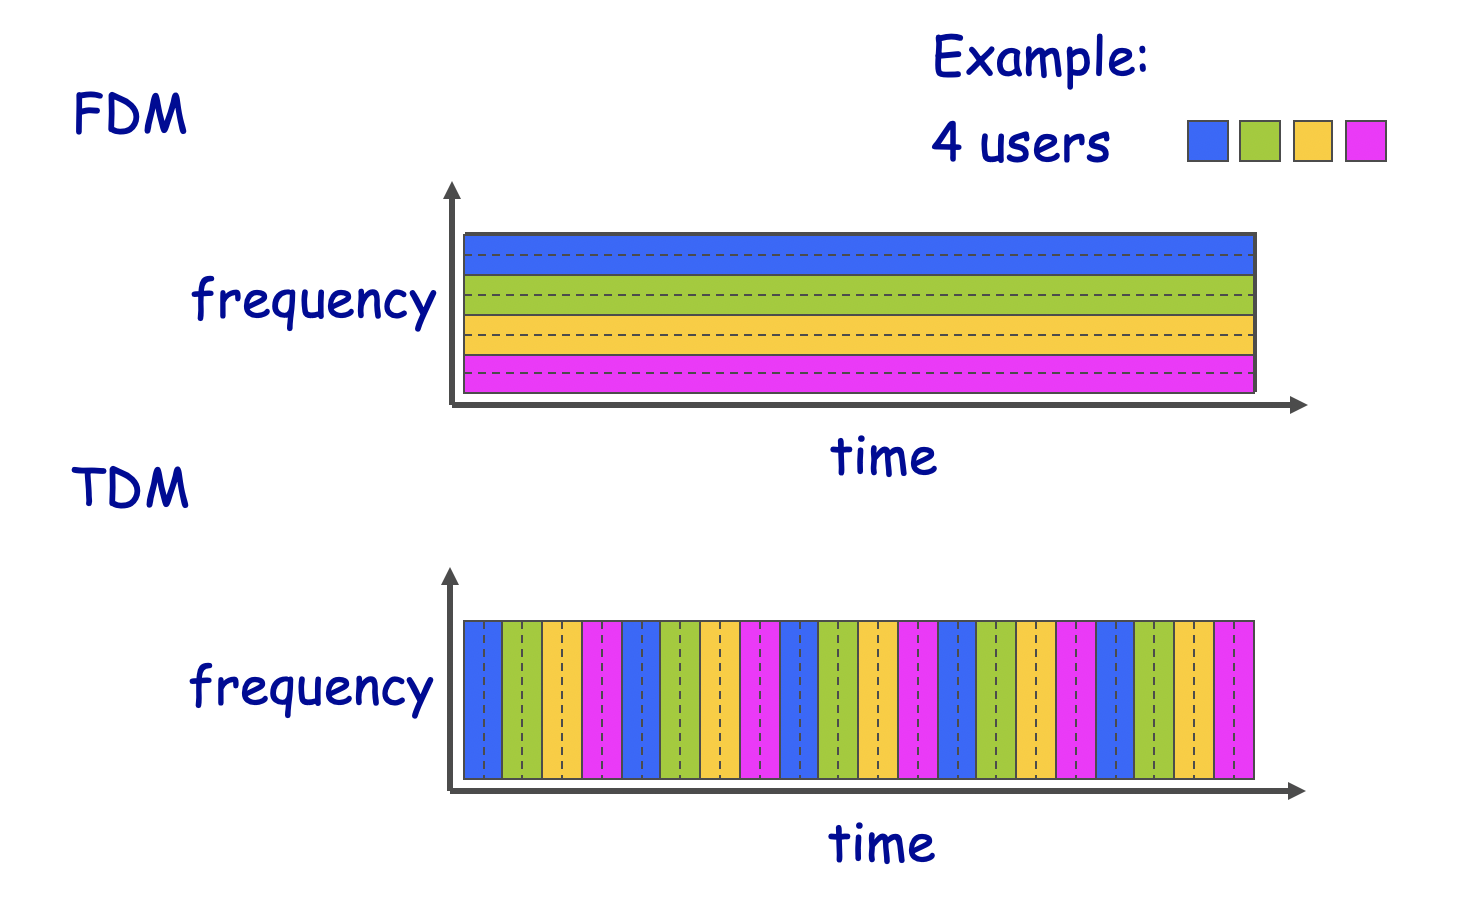
\includegraphics[width=0.8\linewidth]{images/FDMvsTDM.png}
	\caption{FDM versus TDM}
	\label{fig:FDMvsTDM}
\end{figure}

\subsubsection{Trade-off}

Packet Switching is not suitable for real-time services because of its variable and unpredictable end-to-end delays (due primarily to variable and unpredictable queuing delays). Proponents of packet switching argue that (1) it offers better sharing of transmission capacity than circuit switching and (2) it is simpler, more efficient, and less costly to implement than circuit switching.

Circuit switching pre-allocates use of the transmission link \textit{regardless of demand}, with allocated but unneeded link time going unused. Packet switching on the other hand allocates link use \textit{on demand}. Link transmission capacity will be shared on a packet-by-packet basis only among those users who have packets that need to be transmitted over the link.

\subsection{Delay}

Denote $d_{proc}$, $d_{queue}$, $d_{trans}$, and $d_{prop}$ to be the processing, queuing, transmission, and propagation delays respectively. Then the total nodal delay is given by

\[
	d_{nodal} = d_{proc} + d_{queue} + d_{trans} + d_{prop}
\]

\subsubsection{Processing Delay}

The time required to examine the packet’s header and determine where to direct the packet is part of the processing delay.

\subsubsection{Queuing Delay}

Each packet switch has multiple links attached to it. For each attached link, the packet switch has an \textbf{output buffer} (also called an \textbf{output queue}), which stores packets that the router is about to send into that link. If an arriving packet needs to be transmitted onto a link but finds the link busy with the transmission of another packet, the arriving packet must wait in the output buffer. The \textbf{queuing delays} is the time packet waits to be transmitted in the output queue. These delays are variable and depend on the level of congestion in the network. 

Since the amount of buffer space is finite, an arriving packet may find that the buffer is completely full with other packets waiting for transmission. In this case, \textbf{packet loss} will occur --- either the arriving packet or one of the already-queued packets will be dropped.

Denote $a$ to be the average rate at which packets arrive at the queue (in units of packets/sec). The ratio $\frac{aL}{R}$ is called the \textbf{traffic intensity}. If  $\frac{aL}{R} > 1$, then the average rate at which bits arrive at the queue exceeds the rate at which the bits can be transmitted from the queue. In this unfortunate situation, the queue will tend to increase without bound and the queuing delay will approach infinity.

\subsubsection{Transmission Delay}

Most packet switches use \textbf{store-and-forward transmission} at the inputs to the links. Store-and-forward transmission means that the packet switch must receive the entire packet before it can begin to transmit the first bit of the packet onto the outbound link. Consider the general case of sending one packet of $L$ \textit{bits} over a link with rate $R$ \textit{bits/sec}. Then the \textbf{transmission delay} is $\frac{L} {R}$ \textit{seconds}.

\subsubsection{Propagation Delay}

The propagation delay is the distance between two routers divided by the propagation speed. The propagation speed depends on the physical medium of the link and is in the range of $2 \cdot 10^8$ \textit{meters/sec} to $3 \cdot 10^8$ \textit{meters/sec}.

\subsubsection{Clarification}

The \textbf{transmission delay} is the amount of time required for the router to push out the packet; it is a function of the packet’s length and the transmission rate of the link, but has nothing to do with the distance between the two routers. The \textbf{propagation delay}, on the other hand, is the time it takes a bit to propagate from one router to the next; it is a function of the distance between the two routers, but has nothing to do with the packet’s length or the transmission rate of the link.

\subsection{Protocol Layers and Their Service Models}

To provide structure to the design of network protocols, network designers organize protocols—and the network hardware and software that implement the protocols— in \textbf{layers}. We are interested in the \textbf{services} that a layer offers to the layer above—the so-called \textbf{service model} of a layer. When taken together, the protocols of the various layers are called the \textbf{protocol stack}.

\subsection{Security Threats}

\begin{itemize}
	\item \textbf{Denial-of-Service (DoS)}
	\item \textbf{Sniffing}
	\item \textbf{Spoofing}
\end{itemize}

\section{Application Layer}

The application layer is where network applications and their application-layer protocols reside. The Internet's application layer includes many protocols, such as the HTTP, SMTP, FTP and DNS.

\subsection{Transport Services Available to Applications}

\subsubsection{Reliable Data Transfer}

If a protocol provides a guaranteed data delivery service, it is said to provide \textbf{reliable data transfer}. When a transport-layer protocol doesn’t provide reliable data transfer, some of the data sent by the sending process may never arrive at the receiving process. This may be acceptable for \textbf{loss-tolerant applications}.

\subsubsection{Throughput}

A transport-layer protocol may provide guaranteed available throughput at some specified rate. Applications that have throughput requirements are said to be \textbf{bandwidth-sensitive applications}, whereas \textbf{elastic applications} can make use of as much, or as little, throughput as happens to be available.

\subsubsection{Timing}

A transport-layer protocol can also provide timing guarantees.

\subsubsection{Security}

A transport protocol can provide an application with one or more security services.

\subsection{Network Application Architectures}

\subsubsection{Client-Server Architecture}

In a client-server architecture, there is an always-on host, called the \textbf{server}, which services requests from many other hosts, called \textbf{clients}. Often in a client-server application, a single-server host is incapable of keeping up with all the requests from clients. For this reason, a \textbf{data center}, housing a large number of hosts, is often used to create a powerful virtual server. 

\subsubsection{P2P Architecture}

In a P2P architecture, there is minimal (or no) reliance on dedicated servers in data centers. Instead the application exploits direct communication between pairs of intermittently connected hosts, called \textbf{peers}. One of the most compelling features of P2P architectures is their \textbf{self-scalability}. P2P architectures are also cost effective, since they normally don’t require significant server infrastructure and server bandwidth. However, P2P applications face challenges of security, performance, and reliability due to their highly decentralized structure.


\subsection{HTTP : HyperText Transfer Protocol}

HTTP is implemented in two programs: a client program and a server program. The client program and server program, executing on different end systems, talk to each other by exchanging HTTP messages.
HTTP is mainly a \textbf{pull protocol} --- someone loads information on a Web server and users use HTTP to pull the information from the server at their convenience.
Because an HTTP server maintains no information about the clients, HTTP is said to be a \textbf{stateless protocol}.
If each request/response pair be sent over a separate TCP connection, the application is said to use \textbf{non-persistent connections}. If all of the requests and their corresponding responses be sent over the same TCP connection, the application is said to use \textbf{persistent connections}. HTTP can use both non-persistent connections and persistent connections.

\subsubsection{HTTP Request Message}

~\ 

\texttt{GET /somedir/page.html HTTP/1.1}

\texttt{Host: www.someschool.edu}

\texttt{Connection: close}

\texttt{User-agent: Mozilla/5.0}

\texttt{Accept-language: fr}

\begin{figure}[h]
	\centering
	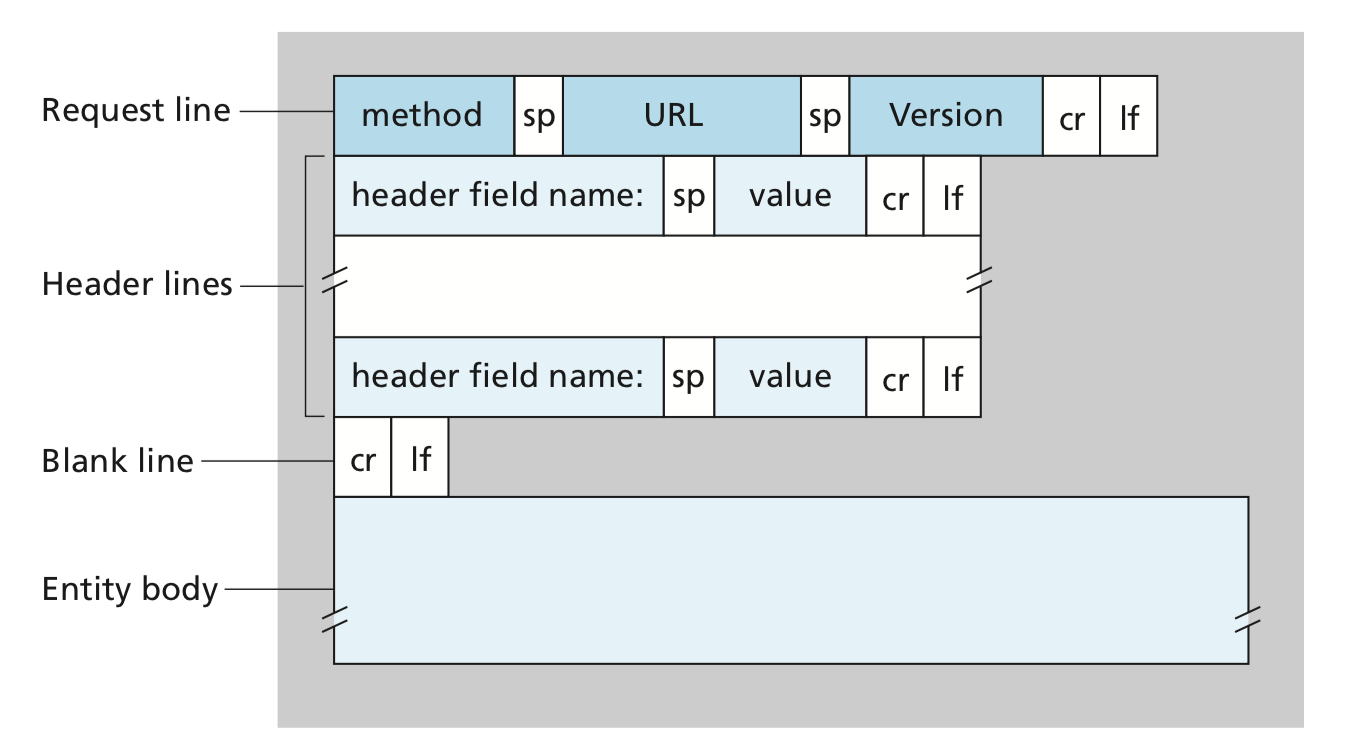
\includegraphics[width=0.8\linewidth]{images/HttpRequest.png}
	\caption{General format of an HTTP request message}
	\label{fig:HttpRequest}
\end{figure}

\subsubsection{HTTP Response Message}

~\

\texttt{HTTP/1.1 200 OK}

\texttt{Connection: close}

\texttt{Date: Tue, 18 Aug 2015 15:44:04 GMT}

\texttt{Server: Apache/2.2.3 (CentOS)}

\texttt{Last-Modified: Tue, 18 Aug 2015 15:11:03 GMT}

\texttt{Content-Length: 6821}

\texttt{Content-Type: text/html}

\begin{figure}[h]
	\centering
	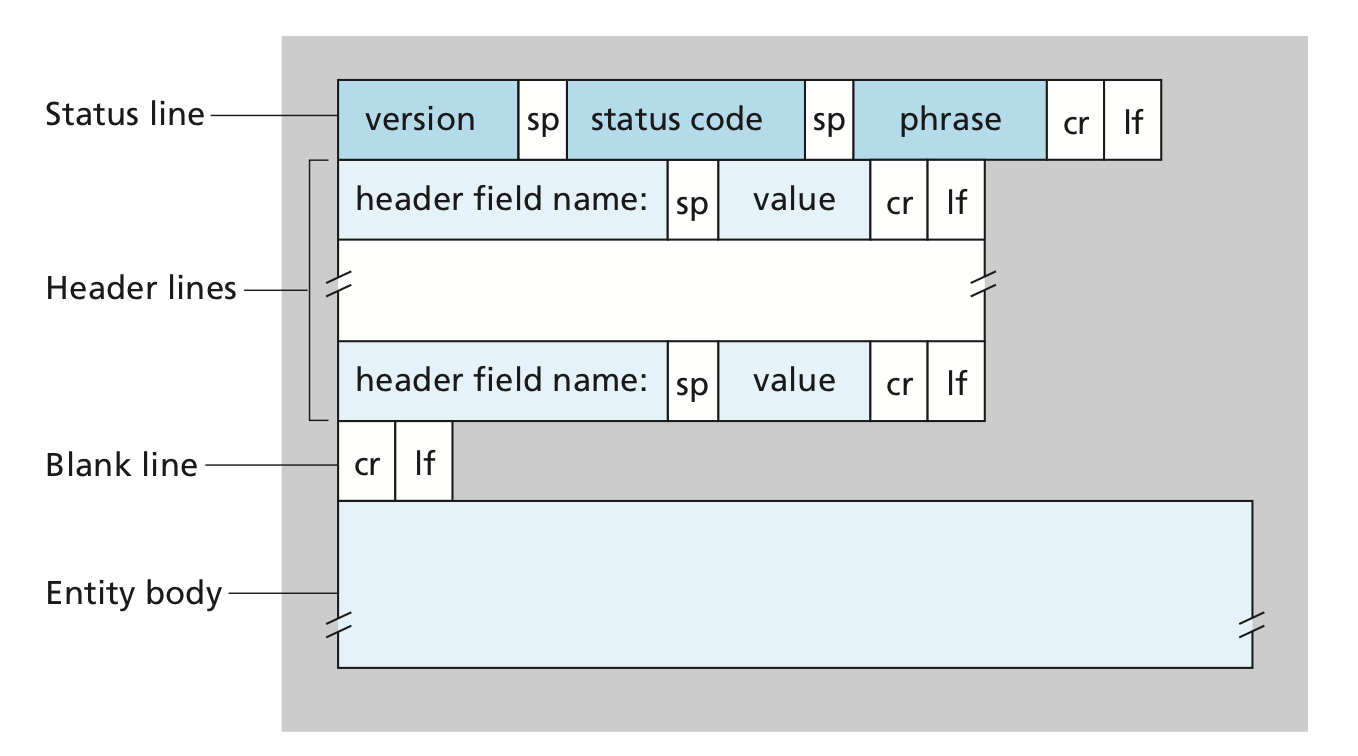
\includegraphics[width=0.8\linewidth]{images/HttpResponse.png}
	\caption{General format of an HTTP response message}
	\label{fig:HttpResponse}
\end{figure}

\subsubsection{Common HTTP Status Codes}

\begin{itemize}
	\item \textbf{200 OK}
	
	Request succeeded and the information is returned in the response.
	
	\item \textbf{301 Moved Permanently}
	
	Requested object has been permanently moved; the new URL is specified in \textit{Location} header of the response message. The client software will automatically retrieve the new URL.
	
	\item \textbf{400 Bad Request}
	
	This is a generic error code indicating that the request could not be understood by the server.
	
	\item \textbf{404 Not Found}
	
	The requested document does not exist on this server.
	
	\item \textbf{505 HTTP Version Not Supported}
	
	 The requested HTTP protocol version is not supported by the server.
	 
\end{itemize}

\subsection{SMTP : Simple Mail Transfer Protocol}

SMTP transfers messages from senders’ mail servers to the recipients’ mail servers.
And it is primarily a \textbf{push protocol} --- the sending mail server pushes the file to the receiving mail server.
Although SMTP has numerous wonderful qualities, it is nevertheless a legacy technology that possesses certain archaic characteristics. For example, it restricts the body (not just the headers) of all mail messages to simple 7-bit ASCII. It requires binary multimedia data to be encoded to ASCII before being sent over SMTP; and it requires the corresponding ASCII message to be decoded back to binary after SMTP transport.

~\

\texttt{telnet serverName 25}

\texttt{S: 220 hamburger.edu}

\texttt{C: HELO crepes.fr}

\texttt{S: 250 Hello crepes.fr, pleased to meet you}

\texttt{C: MAIL FROM: <alice@crepes.fr>}

\texttt{S: 250 alice@crepes.fr ... Sender ok}

\texttt{C: RCPT TO: <bob@hamburger.edu>}

\texttt{S: 250 bob@hamburger.edu ... Recipient ok}

\texttt{C: DATA}

\texttt{S: 354 Enter mail, end with ”.” on a line by itself}

\texttt{C: Do you like ketchup?}

\texttt{C: How about pickles?}

\texttt{C: .}

\texttt{S: 250 Message accepted for delivery}

\texttt{C: QUIT}

\texttt{S: 221 hamburger.edu closing connection}

\subsection{POP3 : Post Office Protocol --- Version 3}

POP3 begins when the user agent opens a TCP connection to the mail server on port 110. With the TCP connection established, POP3 progresses through three phases: authorization, transaction, and update. 

\begin{itemize}
	\item During the first phase, authorization, the user agent sends a username and a password (in the clear) to authenticate the user.
	
	\texttt{telnet mailServer 110}

	\texttt{+OK POP3 server ready}

	\texttt{user bob}

	\texttt{+OK}

	\texttt{pass hungry}

	\texttt{+OK user successfully logged on}
	
	\item During the second phase, transaction, the user agent retrieves messages; also during this phase, the user agent can mark messages for deletion, remove deletion marks, and obtain mail statistics.
	
	\texttt{C: list}
	
	\texttt{S: 1 498 }
	
	\texttt{S: 2 912 }
	
	\texttt{S: .}
	
	\texttt{C: retr 1}
	
	\texttt{S: (blah blah ...}
	
	\texttt{S: .................}
	
	\texttt{S: ..........blah)}
	
	\texttt{S: .}
	
	\texttt{C: dele 1}
	
	\texttt{C: retr 2}
	
	\texttt{S: (blah blah ... }
	
	\texttt{S: .................}
	
	\texttt{S: ..........blah)}
	
	\texttt{S: .}
	
	\texttt{C: dele 2}

	\texttt{C: quit}
	
	\texttt{S: +OK POP3 server signing off}

	
	\item The third phase, update, occurs after the client has issued the quit command, ending the POP3 session; at this time, the mail server deletes the messages that were marked for deletion.
\end{itemize}

\subsection{IMAP : Internet Mail Access Protocol}

An IMAP server will associate each message with a folder; when a message first arrives at the server, it is associated with the recipient’s INBOX folder. The recipient can then move the message into a new, user-created folder, read the message, delete the message, and so on. The IMAP protocol provides commands to allow users to create folders and move messages from one folder to another. IMAP also provides commands that allow users to search remote folders for messages matching specific criteria. Another important feature of IMAP is that it has commands that permit a user agent to obtain components of messages. For example, a user agent can obtain just the message header of a message or just one part of a multipart MIME message.

\subsection{DNS : Domain Name System}

The DNS is (1) a distributed database that translates hostnames to IP addresses and implemented in a hierarchy of DNS servers, and (2) an application-layer protocol that allows hosts to query the distributed database. DNS provides a few other important services in addition to translating hostnames to IP addresses:

\begin{itemize}
	\item \textbf{Host aliasing}
	
	A host with a complicated hostname can have one or more alias names.
	
	\item \textbf{Mail server aliasing}
	
	DNS can be invoked by a mail application to obtain the canonical hostname for a supplied alias hostname as well as the IP address of the host.
	
	\item \textbf{Load distribution}
	
	DNS is also used to perform load distribution among replicated servers, such as replicated Web servers.
\end{itemize}

\subsubsection{Distributed and Hierarchical DNS Structure}

\begin{itemize}
	\item \textbf{Root DNS servers}
	
	Root name servers provide the IP addresses of the TLD servers.
	
	\item \textbf{Top-level domain (TLD) servers}
	
	For each of the top-level domains,  there is TLD server (or server cluster).
	
	\item \textbf{Authoritative DNS servers}
	
	Every organization with publicly accessible hosts (such as Web servers and mail servers) on the Internet must provide publicly accessible DNS records that map the names of those hosts to IP addresses. An organization’s authoritative DNS server houses these DNS records.
	
\end{itemize}

There is another important type of DNS server called the \textbf{local DNS server}. A local DNS server does not strictly belong to the hierarchy of servers but is nevertheless central to the DNS architecture. Each ISP has a local DNS server (also called a default name server). When a host connects to an ISP, the ISP provides the host with the IP addresses of one or more of its local DNS servers. When a host makes a DNS query, the query is sent to the local DNS server, which acts a proxy, forwarding the query into the DNS server hierarchy,

\begin{figure}[h]
	\centering
	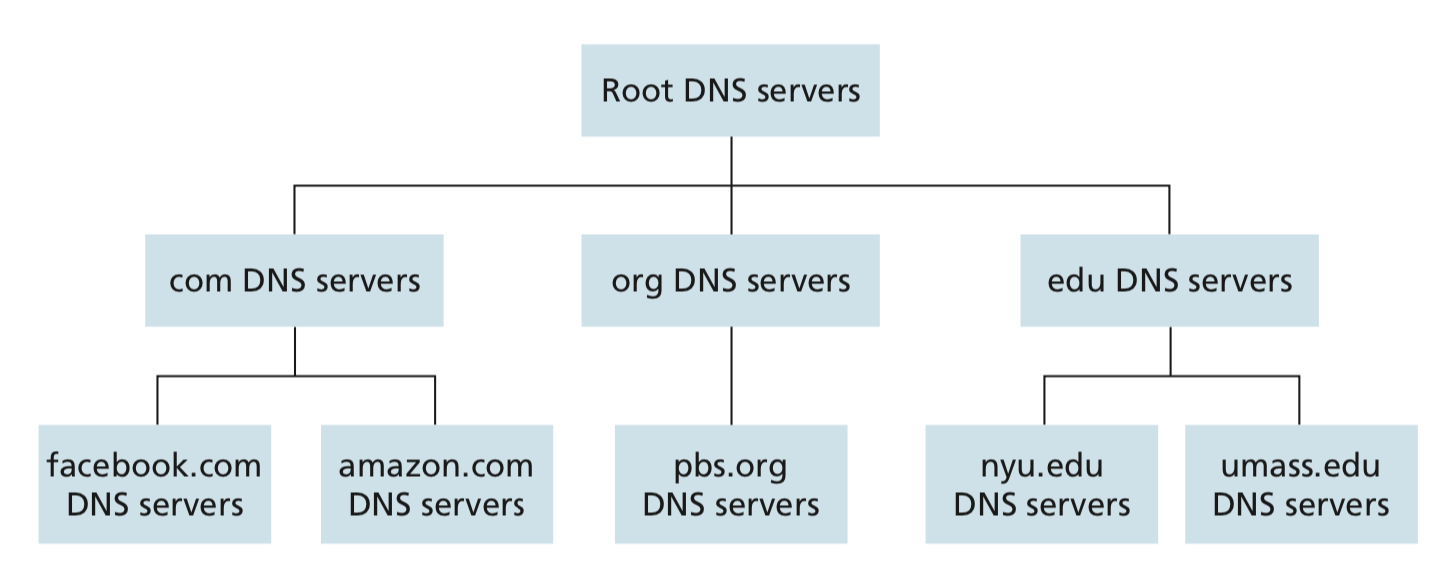
\includegraphics[width=0.8\linewidth]{images/DNS.png}
	\caption{hierarchy of DNS servers}
	\label{fig:DNS}
\end{figure}

\subsubsection{RR : Resource Record}

A resource record is a four-tuple that contains the following fields: 

\texttt{(Name, Value, Type, TTL)}

\texttt{TTL} is the time to live of the resource record; it determines when a resource should be removed from a cache.
The meaning of \texttt{Name} and \texttt{Value} depend on \texttt{Type}:

\begin{itemize}
	\item 
	
	If \texttt{Type=A}, then \texttt{Name} is a hostname and \texttt{Value} is the IP address for the hostname. Thus, a \texttt{Type A} record provides the standard hostname-to-IP address mapping. 
	
	As an example, \texttt{(relay1.bar.foo.com, 145.37.93.126, A)} is a \texttt{Type A} record.
	
	\item
	
	If \texttt{Type=NS}, then \texttt{Name} is a domain (such as foo.com) and \texttt{Value} is the hostname of an authoritative DNS server that knows how to obtain the IP addresses for hosts in the domain. This record is used to route DNS queries further along in the query chain. 
	
	As an example, \texttt{(foo.com, dns.foo.com, NS)} is a \texttt{Type NS} record.
	
	\item
	
	If \texttt{Type=CNAME}, then \texttt{Value} is a canonical hostname for the alias hostname Name. This record can provide querying hosts the canonical name for a hostname. 
	
	As an example, \texttt{(foo.com, relay1.bar.foo.com, CNAME)} is a \texttt{CNAME} record.
	
	\item
	
	If \texttt{Type=MX}, then Value is the canonical name of a mail server that has an alias hostname Name. \texttt{MX} records allow the hostnames of mail servers to have simple aliases.
	
	As an example, \texttt{(foo.com, mail.bar.foo.com, MX)} is an \texttt{MX} record. 
	
\end{itemize}

\subsubsection{DNS Messages}

\begin{itemize}

	\item 
	
	The first 12 bytes is the \textit{header section}, which has a number of fields. The first field is a 16-bit number that identifies the query. This identifier is copied into the reply message to a query, allowing the client to match received replies with sent queries. There are a number of flags in the flag field. A 1-bit query/reply flag indicates whether the message is a query (0) or a reply (1). A 1-bit authoritative flag is set in a reply message when a DNS server is an authoritative server for a queried name. A 1-bit recursion-desired flag is set when a client (host or DNS server) desires that the DNS server perform recursion when it doesn’t have the record. A 1-bit recursion-available field is set in a reply if the DNS server supports recursion. In the header, there are also four number-of fields. These fields indicate the number of occurrences of the four types of data sections that follow the header.
	
	\item
	
	The \textit{question section} contains information about the query that is being made. This section includes (1) a name field that contains the name that is being queried, and (2) a type field that indicates the type of question being asked about the name—for example, a host address associated with a name (\texttt{Type A}) or the mail server for a name (\texttt{Type MX}).
	
	\item
	
	In a reply from a DNS server, the \textit{answer section} contains the resource records for the name that was originally queried.
	
	\item
	
	The \textit{authority section} contains records of other authoritative servers.
	
	\item
	
	The \textit{additional section} contains other helpful records.


\end{itemize}

\begin{figure}[h]
	\centering
	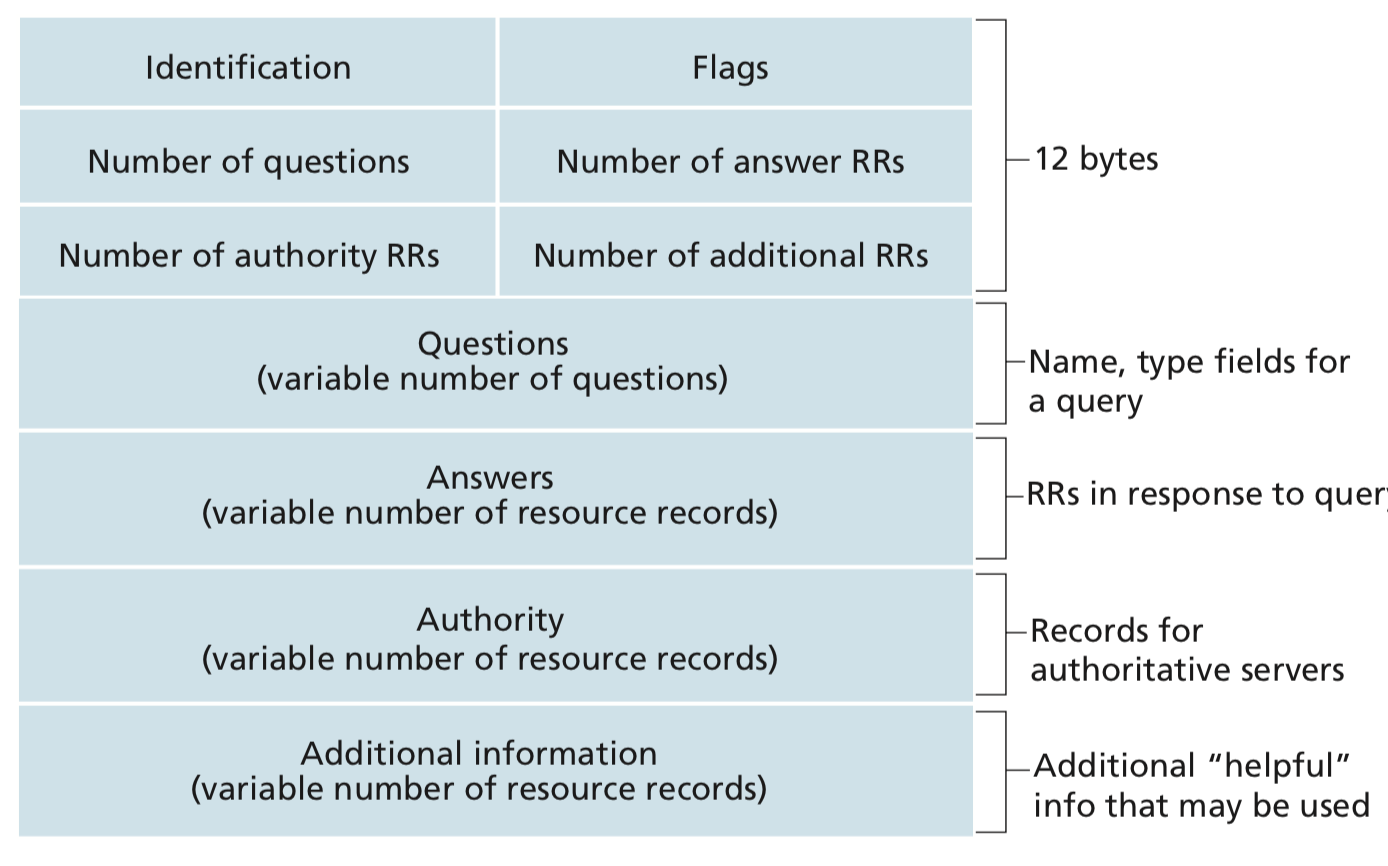
\includegraphics[width=0.8\linewidth]{images/DnsMessage.png}
	\caption{DNS message format}
	\label{fig:DnsMessage}
\end{figure}

\subsection{Peer-to-Peer File Distribution}

Denote the upload rate of the server’s access link by $u_s$, the upload rate of the $i$th peer’s access link by $u_i$, and the download rate of the $i$th peer’s access link by $d_i$. Also denote the size of the file to be distributed (in bits) by $F$ and the number of peers that want to obtain a copy of the file by $N$. 

\subsubsection{Distribution Time for the Client-Server Architecture}

\begin{itemize}
	\item 
	
	The server must transmit one copy of the file to each of the $N$ peers. Thus the server must transmit $NF$ bits. Since the server’s upload rate is $u_s$, the time to distribute the file must be at least $\frac{NF}{u_s}$.
	
	\item
	
	Let $d_{min}$ denote the download rate of the peer with the lowest download rate. The peer with the lowest download rate cannot obtain all $F$ bits of the file in less than $\frac{F}{d_{min}}$ seconds. Thus the minimum distribution time is at least $\frac{F}{d_{min}}$.
	
\end{itemize}

Putting these two observations together, we obtain

\[
	D_{cs} \ge \max \{\frac{NF}{u_s}, \frac{F}{d_{min}} \}
\]

This distribution time increases linearly with the number of peers $N$.

\subsubsection{Distribution Time for the P2P Architecture}

\begin{itemize}
	\item 
	
	At the beginning of the distribution, only the server has the file. To get this file into the community of peers, the server must send each bit of the file at least once into its access link. Thus, the minimum distribution time is at least $\frac{F}{u_s}$.
	
	\item
	
	The peer with the lowest download rate cannot obtain all $F$ bits of the file in less than $\frac{F}{d_{min}}$ seconds. Thus the minimum distribution time is at least $\frac{F}{d_{min}}$.
	
	\item
	
	Finally, observe that the total upload capacity of the system as a whole is equal to the upload rate of the server plus the upload rates of each of the individual peers, that is, $u_{total} = u_s + \sum_{i=1}^N u_i$. The system must deliver (upload) $F$ bits to each of the $N$ peers, thus delivering a total of $NF$ bits. This cannot be done at a rate faster than $u_{total}$. Thus, the minimum distribution time is also at least $\frac{NF}{u_s + \sum_{i=1}^N u_i}$.
	
\end{itemize}

Putting these three observations together, we obtain

\[
	D_{P2P} \ge \max \{\frac{F}{u_s}, \frac{F}{d_{min}}, \frac{NF}{u_s + \sum_{i=1}^N u_i} \}
\]

\begin{figure}[h]
	\centering
	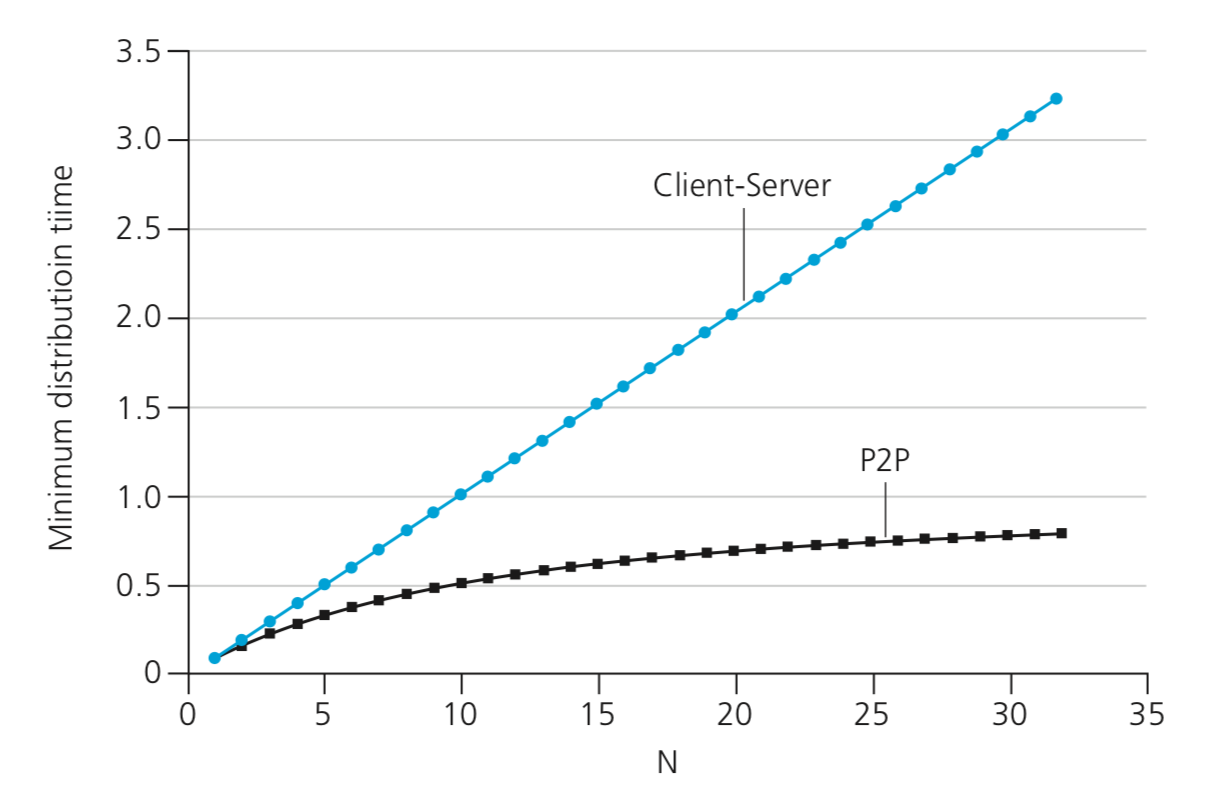
\includegraphics[width=0.8\linewidth]{images/DistributionTime.png}
	\caption{Distribution time for P2P and client-server architectures}
	\label{fig:DistributionTime}
\end{figure}

\subsection{BitTorrent}

BitTorrent is a popular P2P protocol for file distribution. In BitTorrent lingo, the collection of all peers participating in the distribution of a particular file is called a \textbf{torrent}. Peers in a torrent download equal-size \textbf{chunks} of the file from one another, with a typical chunk size of 256 \textit{kbytes}. 

When a peer first joins a torrent, it has no chunks. Over time it accumulates more and more chunks. While it downloads chunks it also uploads chunks to other peers. Once a peer has acquired the entire file, it may (selfishly) leave the torrent, or (altruistically) remain in the torrent and continue to upload chunks to other peers. Also, any peer may leave the torrent at any time with only a subset of chunks, and later rejoin the torrent.

 Each torrent has an infrastructure node called a \textbf{tracker}. When a peer joins a torrent, it registers itself with the tracker and periodically informs the tracker that it is still in the torrent. In this manner, the tracker keeps track of the peers that are participating in the torrent.
 
When a new peer, Alice, joins the torrent, the tracker randomly selects a subset of peers from the set of participating peers, and sends the IP addresses of these 50 peers to Alice. Possessing this list of peers, Alice attempts to establish concurrent TCP connections with all the peers on this list. Let’s call all the peers with which Alice succeeds in establishing a TCP connection ``neighboring peers". At any given time, each peer will have a subset of chunks from the file, with different peers having different subsets. Periodically, Alice will ask each of her neighboring peers for the list of the chunks they have. With this knowledge, Alice will issue requests for chunks she currently does not have.

In deciding which chunks to request, Alice uses a technique called \textbf{rarest first}. The idea is to determine, from among the chunks she does not have, the chunks that are the rarest among her neighbors and then request those rarest chunks first. In this manner, the rarest chunks get more quickly redistributed, aiming to (roughly) equalize the numbers of copies of each chunk in the torrent.

To determine which requests she responds to, BitTorrent uses a clever trading algorithm. The basic idea is that Alice gives priority to the neighbors that are currently supplying her data at the \textbf{highest rate}. Specifically, for each of her neighbors, Alice continually measures the rate at which she receives bits and determines the four peers that are feeding her bits at the highest rate. She then reciprocates by sending chunks to these same four peers. Every 10 seconds, she recalculates the rates and possibly modifies the set of four peers. In BitTorrent lingo, these four peers are said to be \textbf{unchoked}. Importantly, every 30 seconds, she also picks one additional neighbor at random and sends it chunks. Let’s call the randomly chosen peer Bob. In BitTorrent lingo, Bob is said to be \textbf{optimistically unchoked}. Because Alice is sending data to Bob, she may become one of Bob’s top four uploaders, in which case Bob would start to send data to Alice. If the rate at which Bob sends data to Alice is high enough, Bob could then, in turn, become one of Alice’s top four uploaders. In other words, every 30 seconds, Alice will randomly choose a new trading partner and initiate trading with that partner. If the two peers are satisfied with the trading, they will put each other in their top four lists and continue trading with each other until one of the peers finds a better partner. The effect is that peers capable of uploading at compatible rates tend to find each other. The random neighbor selection also allows new peers to get chunks, so that they can have something to trade. All other neighboring peers besides these five peers (four ``top" peers and one probing peer) are ``choked", that is, they do not receive any chunks from Alice.

\subsection{DASH : Dynamic Adaptive Streaming over HTTP}

In DASH, the video is encoded into several different versions, with each version having a different bit rate and, correspondingly, a different quality level. The client dynamically requests chunks of video segments of a few seconds in length. When the amount of available bandwidth is high, the client naturally selects chunks from a high-rate version; and when the available bandwidth is low, it naturally selects from a low-rate version. The client selects different chunks one at a time with HTTP GET request messages.

\subsection{CDNs : Content Distribution Networks}

A CDN manages servers in multiple geographically distributed locations, stores copies of the videos (and other types of Web content, including documents, images, and audio) in its servers, and attempts to direct each user request to a CDN location that will provide the best user experience. CDNs typically adopt one of two different server placement philosophies,

\begin{itemize}

	\item \textbf{Enter Deep}
	
	Deploy server clusters in access ISPs all over the world. The goal is to get close to end users, thereby improving user-perceived delay and throughput by decreasing the number of links and routers between the end user and the CDN server from which it receives content. Because of this highly distributed design, the task of maintaining and managing the clusters becomes challenging.
	
	\item \textbf{Bring Home}
	
	Bring the ISPs home by building large clusters at a smaller number (for example, tens) of sites. Instead of getting inside the access ISPs, these CDNs typically place their clusters in Internet Exchange Points (IXPs). Compared with the enter-deep design philosophy, the bring-home design typically results in lower maintenance and management overhead, possibly at the expense of higher delay and lower throughput to end users.

\end{itemize}

\section{Transport Layer}

A transport-layer protocol provides for \textbf{logical communication} between application processes running on different hosts. By logical communication, we mean that from an application’s perspective, it is as if the hosts running the processes were directly connected; in reality, the hosts may be on opposite sides of the planet, connected via numerous routers and a wide range of link types.

\subsection{Multiplexing and Demultiplexing}

The job of delivering the data in a transport-layer segment to the correct socket is called \textbf{demultiplexing}. The job of gathering data chunks at the source host from different sockets, encapsulating each data chunk with header information to create segments, and passing the segments to the network layer is called \textbf{multiplexing}. A UDP socket is fully identified by a two-tuple consisting of a \textit{destination IP address} and a \textit{destination port number}. A TCP socket is fully identified by its own four-tuple, consisting of \textit{source IP address}, \textit{source port}, \textit{destination IP address} and \textit{destination port}.


\subsection{UDP : User Datagram Protocol}

\subsubsection{Characteristic}

\begin{itemize}
	\item \textbf{Connectionless Service}
	
	\item \textbf{Unreliable Data Transfer Service}
\end{itemize}

\subsubsection{Advantages}

\begin{itemize}
	\item \textbf{Finer application-level control over what and when data is sent}
	
	Under UDP, as soon as an application process passes data to UDP, UDP will package the data inside a UDP segment and immediately pass the segment to the network layer. TCP, on the other hand, has a congestion-control mechanism that throttles the transport-layer TCP sender when one or more links between the source and destination hosts become excessively congested. TCP will also continue to resend a segment until the receipt of the segment has been acknowledged by the destination, regardless of how long reliable delivery takes.
	
	\item \textbf{No connection establishment}
	
	TCP uses a three-way hand- shake before it starts to transfer data. UDP just blasts away without any formal preliminaries. Thus UDP does not introduce any delay to establish a connection.
	
	\item \textbf{No connection state}
	
	TCP maintains connection state in the end systems. This connection state includes receive and send buffers, congestion-control parameters, and sequence and acknowledgment number parameters. UDP, on the other hand, does not maintain connection state and does not track any of these parameters. For this reason, a server devoted to a particular application can typically support many more active clients when the application runs over UDP rather than TCP.
	
	\item \textbf{Small packet header overhead}
	
	The TCP segment has 20 bytes of header overhead in every segment, whereas UDP has only 8 bytes of overhead.
\end{itemize}

\subsubsection{UDP Structure}

The UDP \textbf{checksum} provides for error detection. UDP at the sender side performs the 1s complement of the sum of all the 16-bit words in the segment, with any overflow encountered during the sum being wrapped around. The 1s complement is obtained by converting all the 0s to 1s and converting all the 1s to 0s. At the receiver, all four 16-bit words are added, including the checksum. If no errors are introduced into the packet, then clearly the sum at the receiver will be 1111111111111111. If one of the bits is a 0, then we know that errors have been introduced into the packet.

\begin{figure}[h]
	\centering
	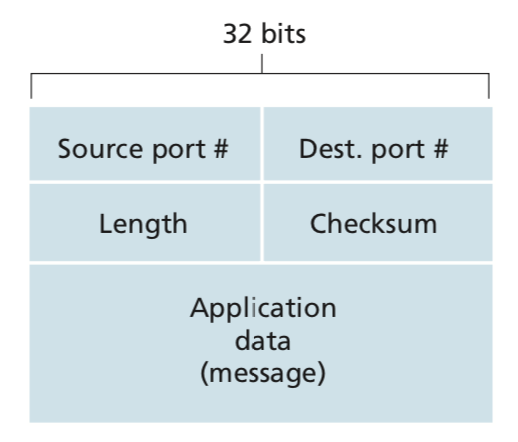
\includegraphics[width=0.4\linewidth]{images/udp.png}
	\caption{UDP segment structure}
	\label{fig:udp}
\end{figure}

\subsection{Principles of Reliable Data Transfer}

TCP’s error-recovery mechanism is probably best categorized as a hybrid of GBN and SR protocols.

\subsubsection{GBN : Go-Back-N}

In a Go-Back-N (GBN) protocol, the sender is allowed to transmit multiple packets without waiting for an acknowledgment, but is constrained to have no more than some maximum allowable number, $N$, of unacknowledged packets in the pipeline.

\begin{figure}[h]
	\centering
	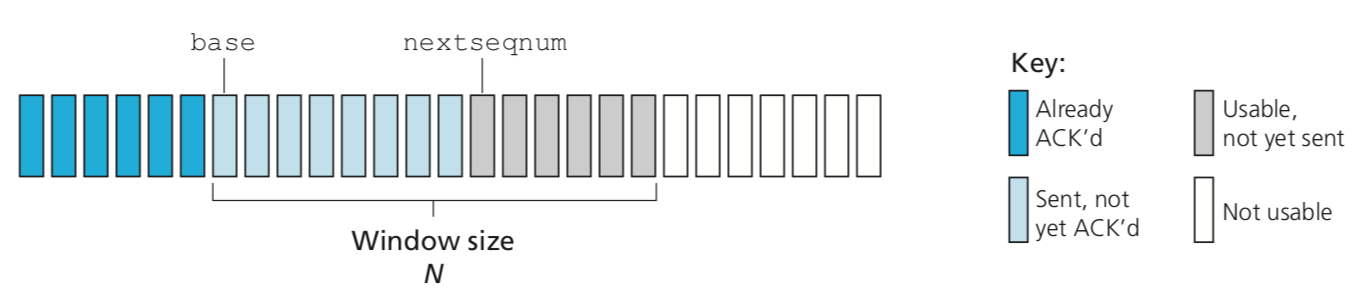
\includegraphics[width=0.8\linewidth]{images/GBN.png}
	\caption{Sender’s view of sequence numbers in Go-Back-N}
	\label{fig:GBN}
\end{figure}

The receiver’s actions in GBN are also simple. If a packet with sequence number $n$ is received correctly and is in order (that is, the data last delivered to the upper layer came from a packet with sequence number $n - 1$), the receiver sends an ACK for packet $n$ and delivers the data portion of the packet to the upper layer. In all other cases, the receiver discards the packet and resends an ACK for the most recently received in-order packet. The use of \textbf{cumulative acknowledgments} is a natural choice for GBN.

\subsubsection{SR : Selective Repeat}

As the name suggests, selective-repeat protocols avoid unnecessary retransmissions by having the sender retransmit only those packets that it suspects were received in error at the receiver. This individual, as-needed, retransmission will require that the receiver \textbf{individually acknowledge} correctly received packets. A window size of $N$ will again be used to limit the number of outstanding, unacknowledged packets in the pipeline.

\begin{figure}[h]
	\centering
	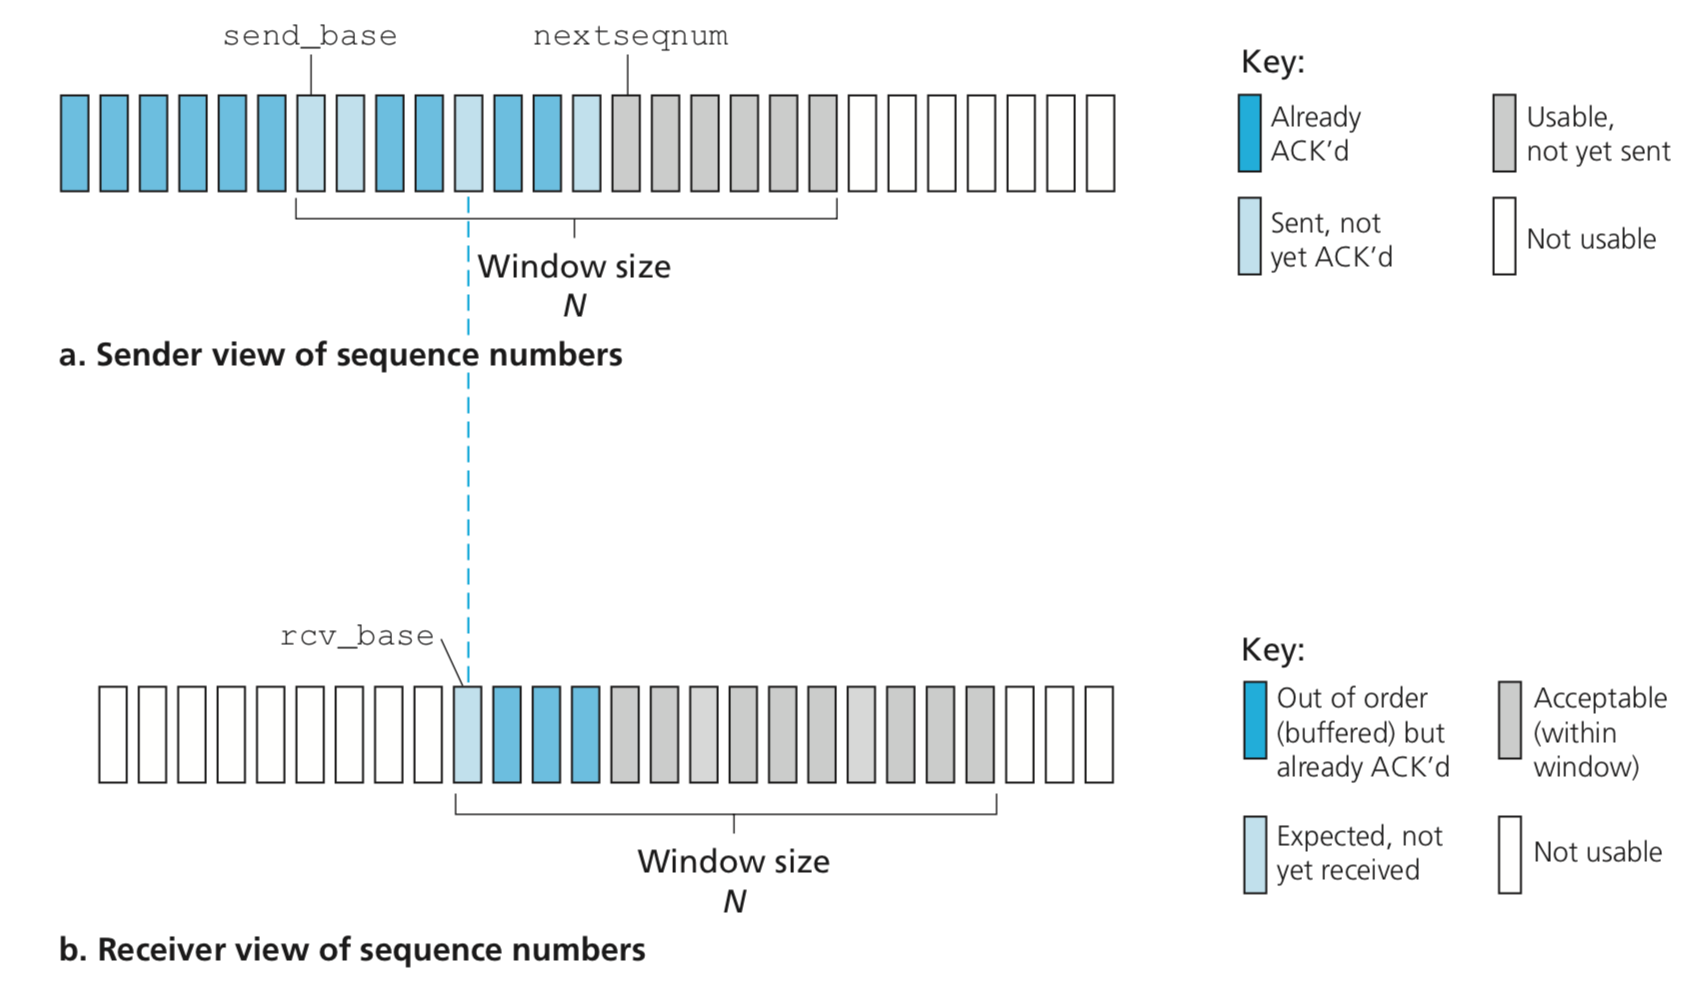
\includegraphics[width=0.8\linewidth]{images/SR.png}
	\caption{Selective-repeat (SR) sender and receiver views of sequence-number space}
	\label{fig:SR}
\end{figure}

\subsection{TCP : Transmission Control Protocol}

\subsubsection{Characteristic}

\begin{itemize}
	\item \textbf{Connection-Oriented Service}
	
	\item \textbf{Reliable Data Transfer Service}
	
	\item \textbf{Full-Duplex Service}
	
	If there is a TCP connection between Process A on one host and Process B on another host, then application-layer data can flow from Process A to Process B at the same time as application-layer data flows from Process B to Process A.
\end{itemize}

\subsubsection{TCP Structure}

\begin{itemize}
	\item
	
	The 32-bit \textbf{sequence number field} and the 32-bit \textbf{acknowledgment number field} are used by the TCP sender and receiver in implementing a reliable data transfer service.
	
	\item 
	
	The 16-bit \textbf{receive window field} is used for flow control.
	
	\item
	
	The 4-bit \textbf{header length field} specifies the length of the TCP header in 32-bit words. The TCP header can be of variable length due to the TCP options field. Typically, the options field is empty, so that the length of the typical TCP header is 20 bytes.
	
	\item
	
	The optional and variable-length \textbf{options field} is used when a sender and receiver negotiate the maximum segment size (MSS) or as a window scaling factor for use in high-speed networks. A time-stamping option is also defined.
	
	\item
	
	The \textbf{ACK} bit is used to indicate that the value carried in the acknowledgment field is valid.
	
	\item
	
	The \textbf{RST}, \textbf{SYN}, and \textbf{FIN} bits are used for connection setup and teardown.
	
	\item
	
	The \textbf{CWR} and \textbf{ECE} bits are used in explicit congestion notification.
	
	\item 
	
	Setting the \textbf{PSH} bit indicates that the receiver should pass the data to the upper layer immediately.
	
	\item
	
	The \textbf{URG} bit is used to indicate that there is data in this segment that the sending-side upper-layer entity has marked as ``urgent". The location of the last byte of this urgent data is indicated by the 16-bit \textbf{urgent data pointer field}. 

\end{itemize}

\begin{figure}[h]
	\centering
	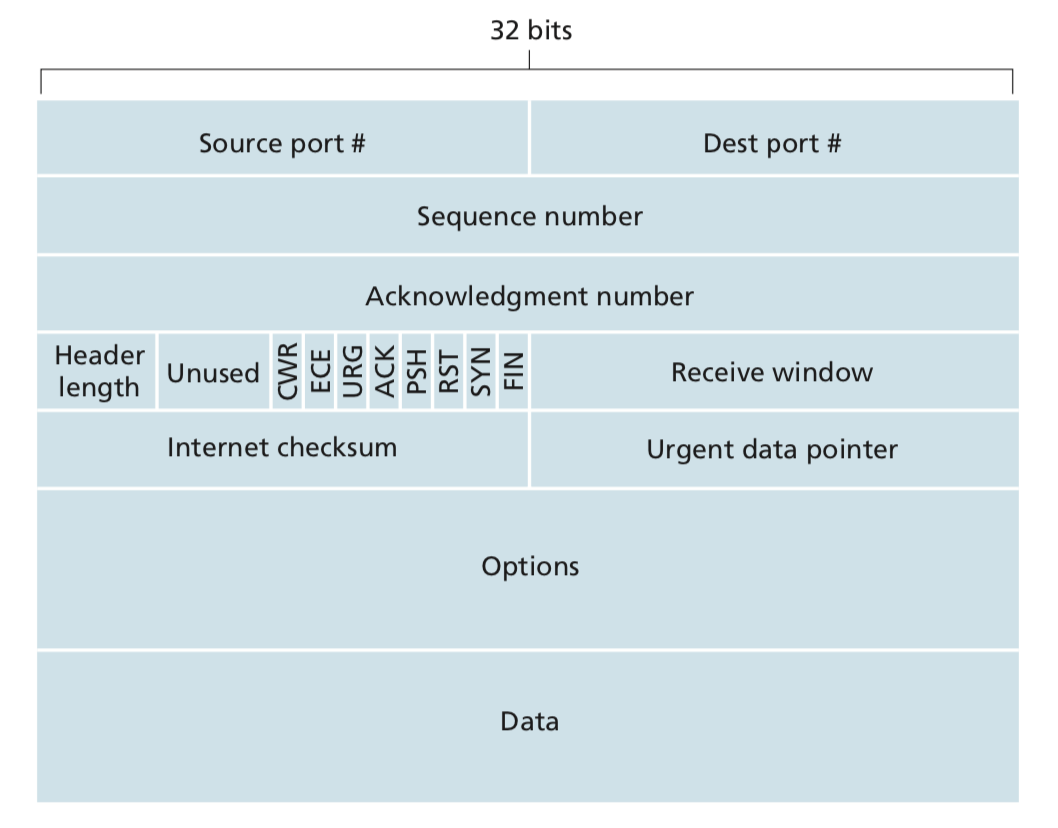
\includegraphics[width=0.8\linewidth]{images/tcp.png}
	\caption{TCP segment structure}
	\label{fig:tcp}
\end{figure}

\subsubsection{Sequence Numbers and Acknowledgment Numbers}

\begin{itemize}

	\item 
	
	The \textbf{sequence number} for a segment is therefore the byte-stream number of the first byte in the segment. 
	
	\item 
	
	The \textbf{acknowledgment number} that Host A puts in its segment is the sequence number of the next byte Host A is expecting from Host B. Thus, TCP is said to provide \textbf{cumulative acknowledgments}.
\end{itemize}

\subsubsection{Round-Trip Time Estimation and Timeout}

\[
	\mathrm{EstimatedRTT} = (1 - \alpha) \cdot \mathrm{EstimatedRTT} + \alpha \cdot \mathrm{SampleRTT}
\]

\textbf{EstimatedRTT} is an \textbf{exponential weighted moving average (EWMA)} of the \textbf{SampleRTT} values. The recommended value of $\alpha$ is 0.125.

\[
	\mathrm{DevRTT} = (1– \beta) \cdot \mathrm{DevRTT} + \beta \cdot | \mathrm{SampleRTT} - \mathrm{EstimatedRTT} |
\]

\textbf{DevRTT} is an \textbf{EWMA} of the difference between \textbf{SampleRTT} and \textbf{EstimatedRTT}. The recommended value of $\beta$ is 0.25.

\[
	\mathrm{TimeoutInterval} = \mathrm{EstimatedRTT} + 4 \cdot \mathrm{DevRTT}
\]

An initial \textbf{TimeoutInterval} value of 1 second is recommended. Also, when a timeout occurs, the value of \textbf{TimeoutInterval} is doubled to avoid a premature timeout occurring for a subsequent segment that will soon be acknowledged. However, as soon as a segment is received and \textbf{EstimatedRTT} is updated, the TimeoutInterval is again computed using the formula above.

\subsubsection{Three-way Handshake}

\begin{figure}[h]
	\centering
	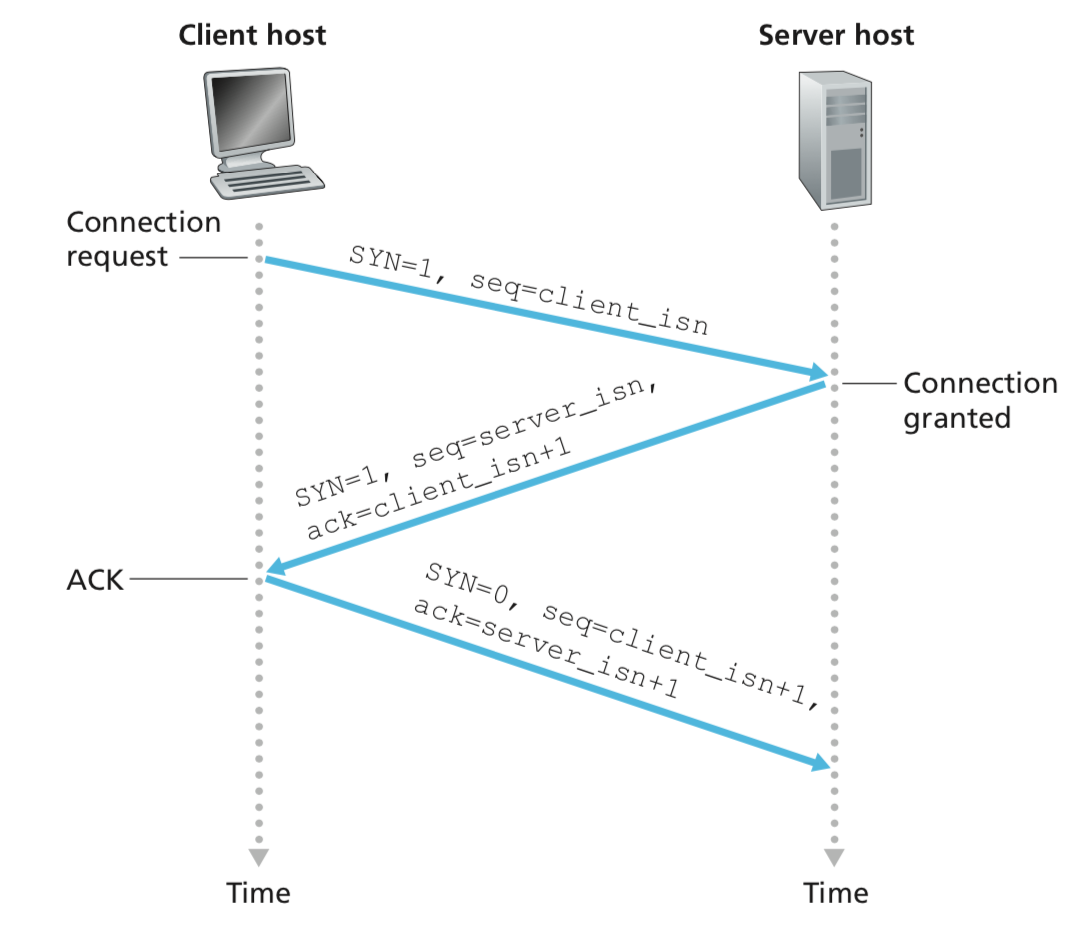
\includegraphics[width=0.6\linewidth]{images/Three-wayHandshake.png}
	\caption{TCP three-way handshake: segment exchange}
	\label{fig:Three-wayHandshake}
\end{figure}

\subsubsection{Flow Control}

TCP provides a \textbf{flow-control service} to its applications to eliminate the possibility of the sender overflowing the receiver’s buffer. TCP provides flow control by having the sender maintain a variable called the \textbf{receive window}.

\begin{figure}[h]
	\centering
	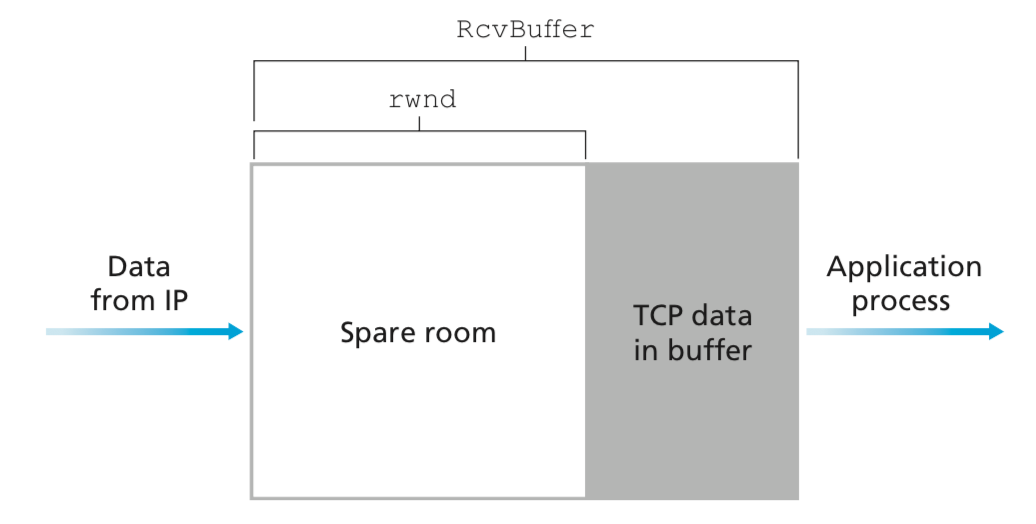
\includegraphics[width=0.8\linewidth]{images/rwnd.png}
	\caption{The receive window (rwnd) and the receive buffer (RcvBuffer)}
	\label{fig:rwnd}
\end{figure}

\subsubsection{Congestion Control --- Additive-increase, Multiplicative-decrease (AIMD)}

\begin{figure}[h]
	\centering
	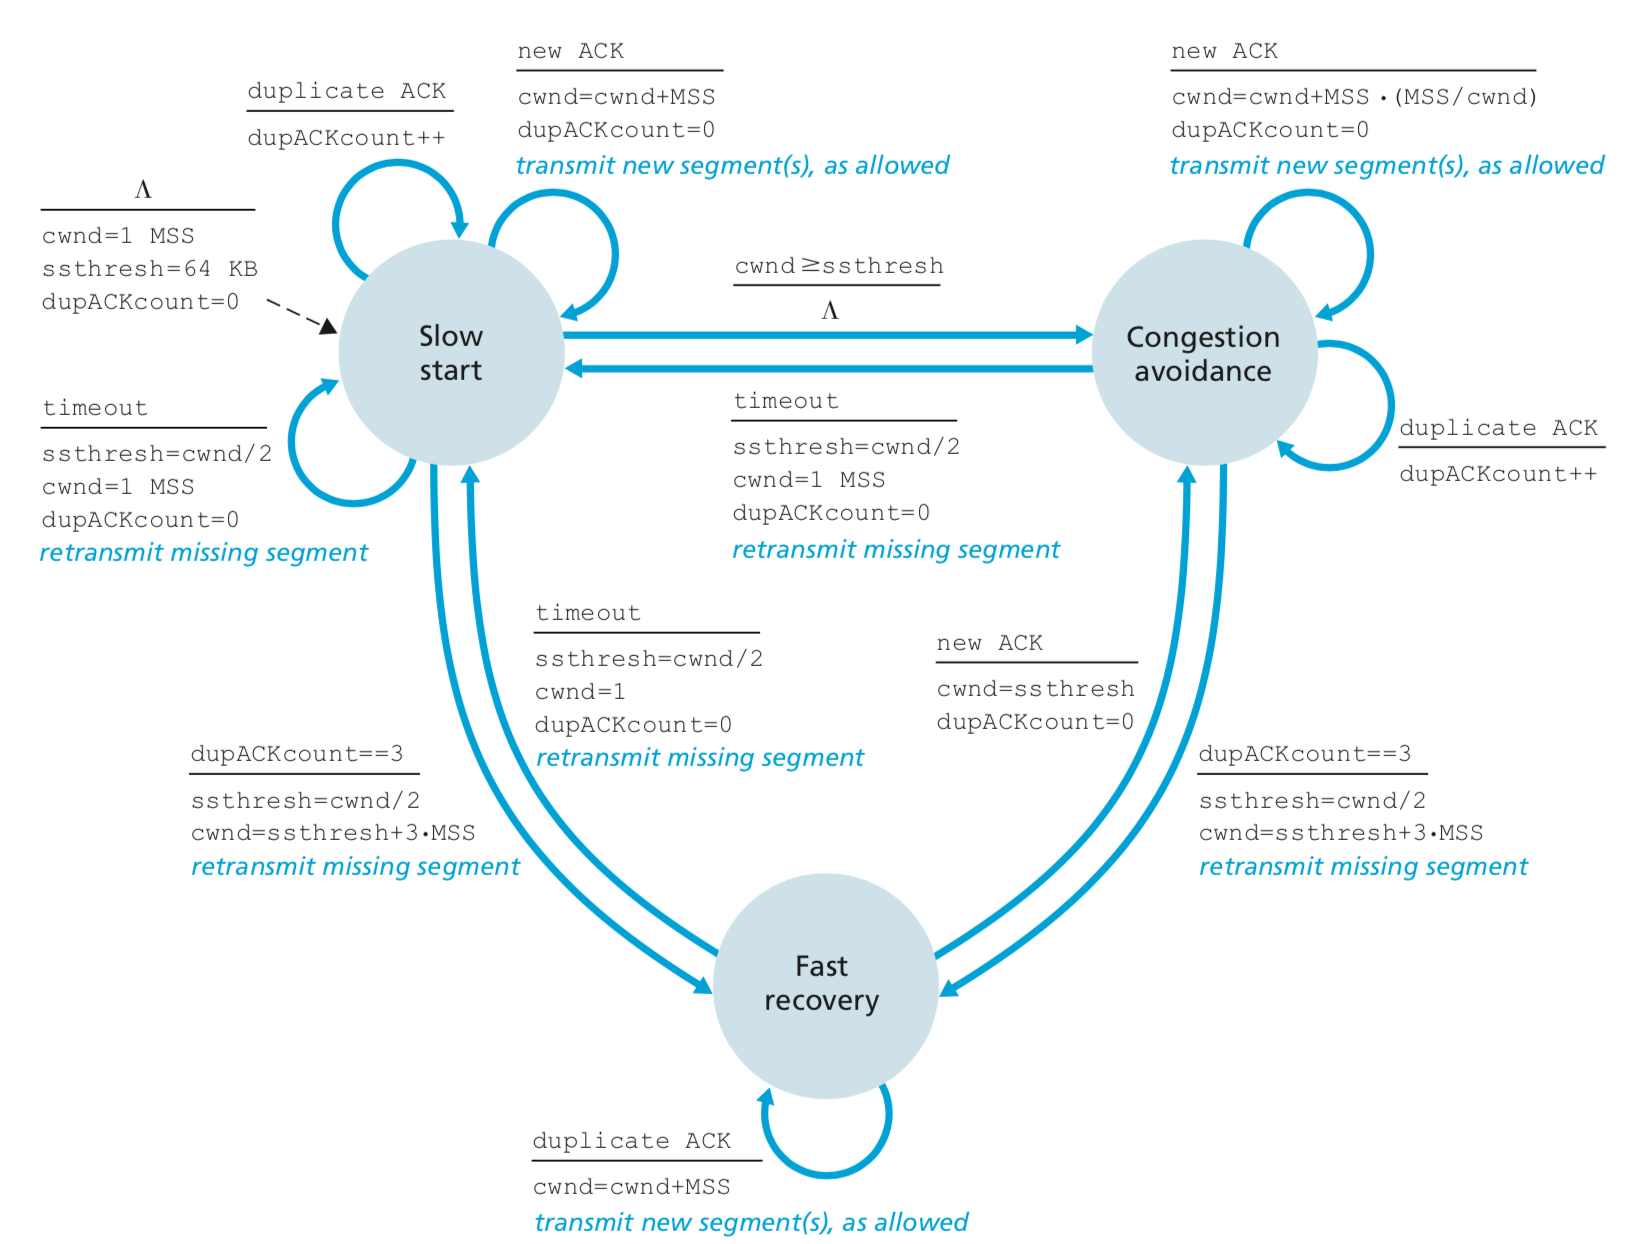
\includegraphics[width=0.9\linewidth]{images/CongestionControl.png}
	\caption{FSM description of TCP congestion control}
	\label{fig:CongestionControl}
\end{figure}

\section{Network Layer}

The Internet’s network layer provides a single service, known as \textbf{best-effort service}. With best-effort service, packets are neither guaranteed to be received in the order in which they were sent, nor is their eventual delivery even guaranteed. There is no guarantee on the end-to-end delay nor is there a minimal bandwidth guarantee. It might appear that best-effort service is a euphemism for \textbf{no service at all}.

\subsection{Control Plane}

\begin{itemize}
	\item \textbf{The Traditional Approach}
	
	A routing algorithm runs in each and every router and both forwarding and routing functions are contained within a router. 
	
	\item \textbf{The SDN Approach}
	
	A physically separate remote controller computes and distributes the forwarding tables to be used by each and every router.
	
\end{itemize}

\subsection{Switching}

\begin{itemize}
	\item \textbf{Switching via memory}
	
	Switching between input and output ports being done under direct control of the CPU. Input and output ports functioned as traditional I/O devices in a traditional operating system. An input port with an arriving packet first signaled the routing processor via an interrupt. The packet was then copied from the input port into processor memory. The routing processor then extracted the destination address from the header, looked up the appropriate output port in the forwarding table, and copied the packet to the output port’s buffers. Note also that \textbf{two packets cannot be forwarded at the same time}, even if they have different destination ports, since only one memory read/write can be done at a time over the shared system bus.
	
	\item \textbf{Switching via a bus}
	
	In this approach, an input port transfers a packet directly to the output port over a shared bus, without intervention by the routing processor. This is typically done by having the input port pre-pend a switch-internal label (header) to the packet indicating the local output port to which this packet is being transferred and transmitting the packet onto the bus. All output ports receive the packet, but only the port that matches the label will keep the packet. The label is then removed at the output port, as this label is only used within the switch to cross the bus. If multiple packets arrive to the router at the same time, each at a different input port, all but one must wait since only one packet can cross the bus at a time. Thus,  \textbf{two packets cannot be forwarded at the same time}.
	
	\item \textbf{Switching via an interconnection network}
	
	A crossbar switch is an interconnection network consisting of $2N$ buses that connect $N$ input ports to $N$ output ports. Each vertical bus intersects each horizontal bus at a crosspoint, which can be opened or closed at any time by the switch fabric controller. Unlike the previous two switching approaches, crossbar switches are \textbf{capable of forwarding multiple packets in parallel}. However, if two packets from two different input ports are destined to that same output port, then one will have to wait at the input, since only one packet can be sent over any given bus at a time.
	
\end{itemize}

\begin{figure}[h]
	\centering
	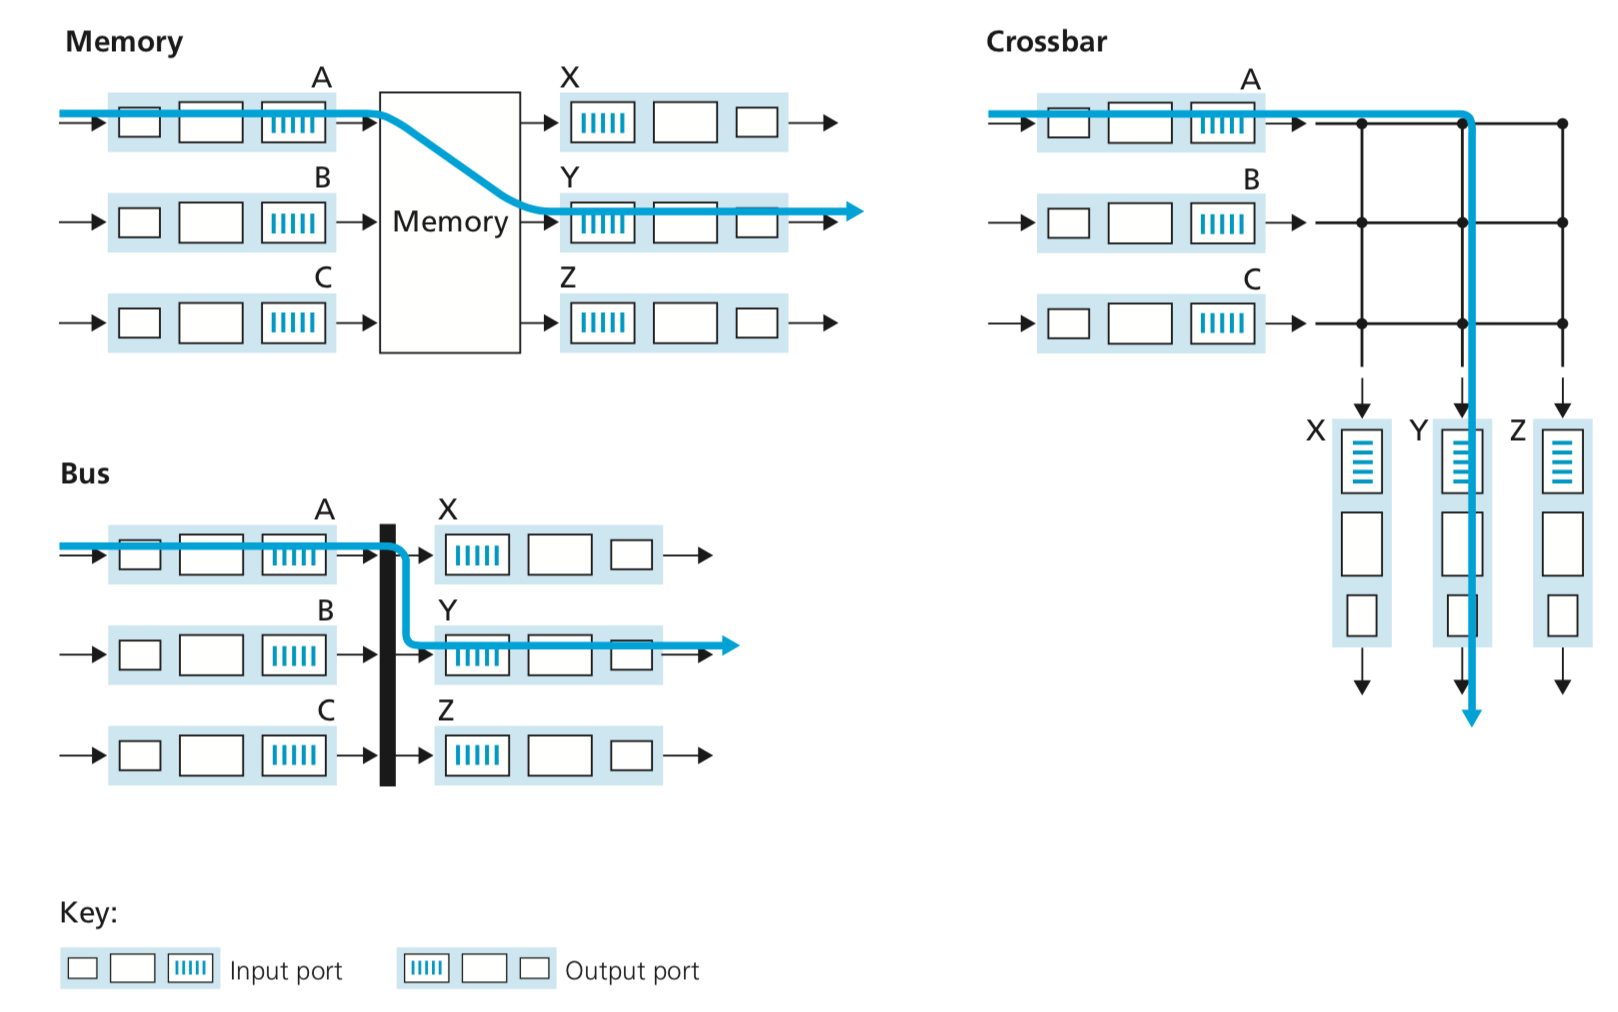
\includegraphics[width=0.8\linewidth]{images/switching.png}
	\caption{Three switching techniques}
	\label{fig:switching}
\end{figure}



\subsection{Input Queueing}

Figure \ref{fig:hol} shows an example in which two packets (darkly shaded) at the front of their input queues are destined for the same upper-right output port. Suppose that the switch fabric chooses to transfer the packet from the front of the upper-left queue. In this case, the darkly shaded packet in the lower-left queue must wait. But not only must this darkly shaded packet wait, so too must the lightly shaded packet that is queued behind that packet in the lower-left queue, even though there is no conten- tion for the middle-right output port (the destination for the lightly shaded packet). This phenomenon is known as head-of-the-line (HOL) blocking in an input-queued switch—a queued packet in an input queue must wait for transfer through the fabric (even though its output port is free) because it is blocked by another packet at the head of the line. 

\begin{figure}[h]
	\centering
	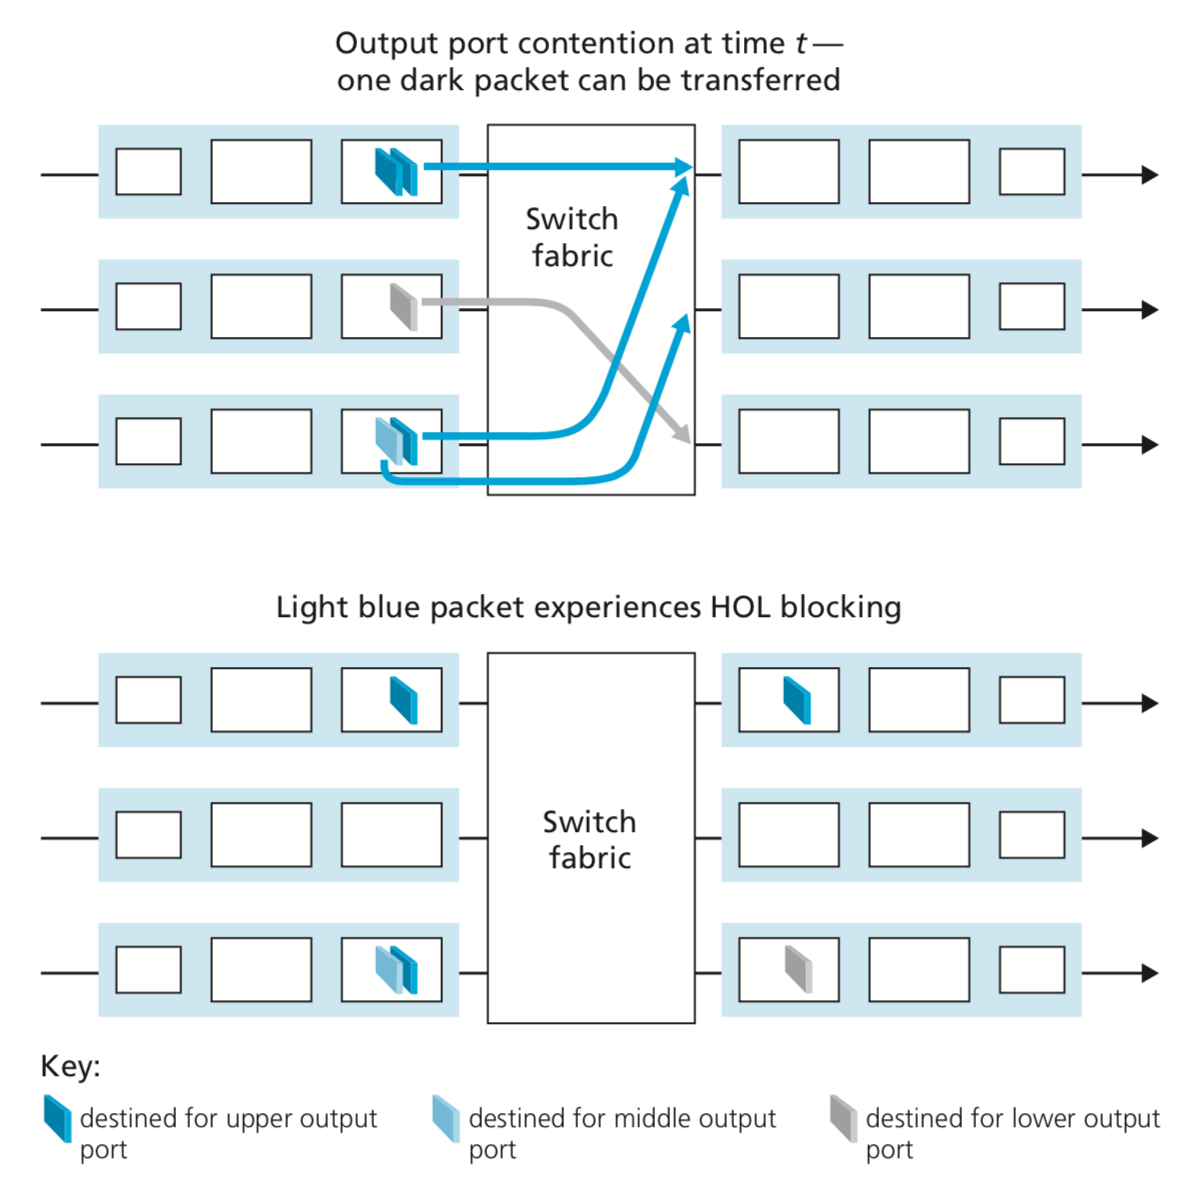
\includegraphics[width=0.8\linewidth]{images/hol.png}
	\caption{HOL blocking at and input-queued switch}
	\label{fig:hol}
\end{figure}

\subsection{Packet Scheduling}

\begin{itemize}
	\item \textbf{First-in-First-Out (FIFO)}
	
	\item \textbf{Priority Queuing}
	
	\item \textbf{Round Robin and Weighted Fair Queuing (WFQ)}
\end{itemize}


\subsection{The Internet Protocol Version 4}

\begin{itemize}
	
	\item \textbf{Version number}
	
	 These 4 bits specify the IP protocol version of the datagram.
	 
	 \item \textbf{Header length}
	 
	  Because an IPv4 datagram can contain a variable number of options, these 4 bits are needed to determine where in the IP datagram the payload actually begins. Most IP datagrams do not contain options, so the typical IP datagram has a \textbf{20-byte header}.
	  
	  \item \textbf{Type of service}
	  
	  The type of service (TOS) bits were included in the IPv4 header to allow different types of IP datagrams to be distinguished from each other.
	  
	  \item \textbf{Datagram length}
	  
	  This is the total length of the IP datagram (header plus data), measured in bytes.
	  
	  \item \textbf{Identifier, flags, fragmentation offset}
	  
	  These three fields have to do with so-called IP fragmentation.
	  
	  \item \textbf{Time-to-live}
	  
	  The time-to-live field is included to ensure that datagrams do not circulate forever in the network. This field is decremented by one each time the datagram is processed by a router. If the TTL field reaches 0, a router must drop that datagram.
	  
	  \item \textbf{Protocol}
	  
	  This field is typically used only when an IP datagram reaches its final destination. The value of this field indicates the specific transport-layer protocol to which the data portion of this IP datagram should be passed. For example, a value of 6 indicates that the data portion is passed to TCP, while a value of 17 indicates that the data is passed to UDP.
	   
	  \item \textbf{Header checksum}
	  
	  The header checksum aids a router in detecting bit errors in a received IP datagram. The header checksum is computed by treating each 2 bytes in the header as a number and summing these numbers using 1s complement arithmetic. 
	    
	  \item \textbf{Source and destination IP addresses}
	  
	  When a source creates a datagram, it inserts its IP address into the source IP address field and inserts the address of the ultimate destination into the destination IP address field.
	  
	  \item \textbf{Options}
	  
	  The options fields allow an IP header to be extended. Header options were meant to be used rarely.
	  
	  \item \textbf{Data (payload)}
	  
	  The data field of the IP datagram contains the transport-layer segment (TCP or UDP) to be delivered to the destination.
	
\end{itemize}

\begin{figure}[h]
	\centering
	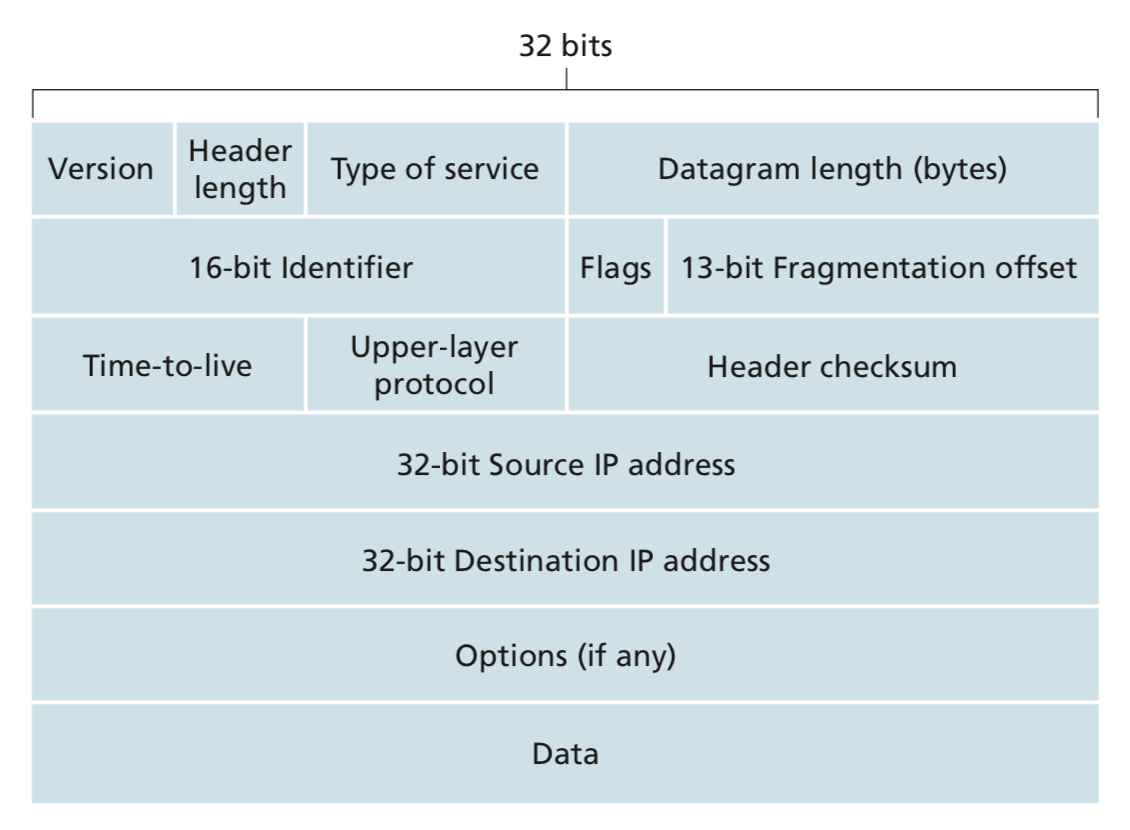
\includegraphics[width=0.7\linewidth]{images/ipv4.png}
	\caption{IPv4 datagram format}
	\label{fig:ipv4}
\end{figure}

\subsection{IPv4 Addressing}

An IP address is technically associated with an interface, rather than with the host or router containing that interface. Addresses are typically written in so-called \textbf{dotted-decimal notation}, in which each byte of the address is written in its decimal form and is separated by a period (dot) from other bytes in the address. 

To determine the subnets, detach each interface from its host or router, creating islands of isolated networks, with interfaces terminating the end points of the isolated networks. Each of these isolated networks is called a \textbf{subnet}. 

The Internet’s address assignment strategy is known as \textbf{Classless Interdomain Routing} (CIDR—pronounced cider). CIDR generalizes the notion of subnet addressing. As with subnet addressing, the 32-bit IP address is divided into two parts and again has the dotted-decimal form $a.b.c.d/x$, where $x$ indicates the number of bits in the first part of the address.

Before CIDR was adopted, the network portions of an IP address were constrained to be 8, 16, or 24 bits in length, an addressing scheme known as \textbf{classful addressing}, since subnets with 8-, 16-, and 24-bit subnet addresses were known as class A, B, and C networks, respectively. The requirement that the subnet portion of an IP address be exactly 1, 2, or 3 bytes long turned out to be problematic for supporting the rapidly growing number of organizations with small and medium-sized subnets.

Also, when a host sends a datagram with destination address $255.255.255.255$, the message is delivered to all hosts on the same subnet. It is called \textbf{broadcast address}

\subsection{DHCP : The Dynamic Host Configuration Protocol}

\begin{figure}[h]
	\centering
	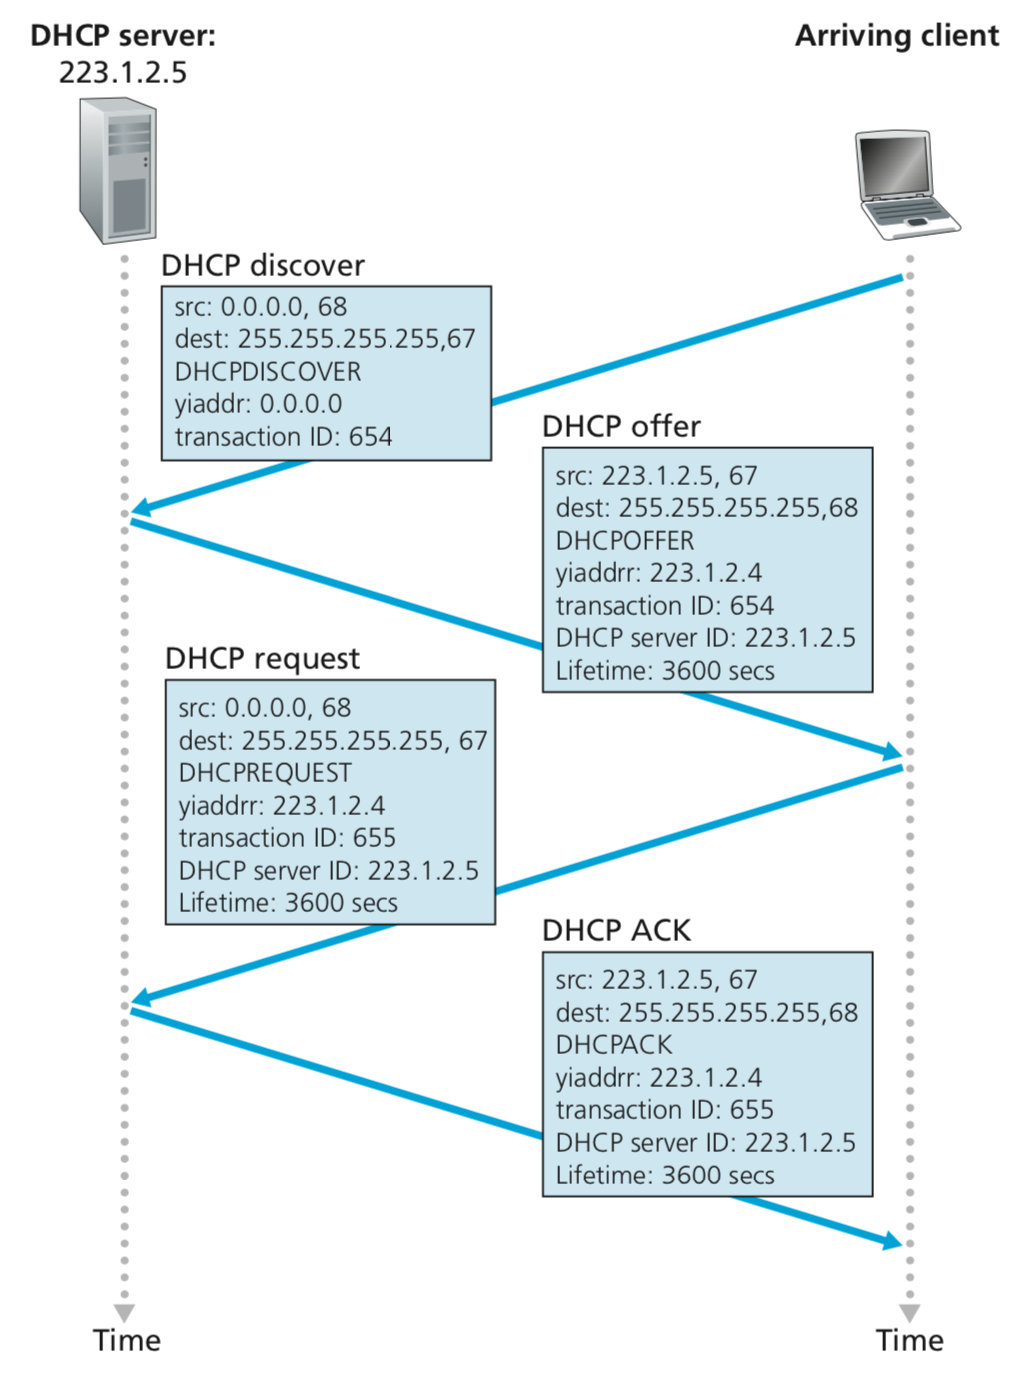
\includegraphics[width=0.45\linewidth]{images/DHCP.png}
	\caption{DHCP client-server interaction}
	\label{fig:DHCP}
\end{figure}

\begin{itemize}
	\item \textbf{DHCP server discovery}
	
	The first task of a newly arriving host is to find a DHCP server with which to interact. This is done using a DHCP discover message, which a client sends within a UDP packet to port 67 with broadcast destination IP address.
	
	\item \textbf{DHCP server offer(s)}
	
	A DHCP server receiving a DHCP discover message responds to the client with a DHCP offer message, which is also sent to broadcast IP address.
	
	\item \textbf{DHCP request}

	The newly arriving client will choose from among one or more server offers and respond to its selected offer with a DHCP request message, echoing back the configuration parameters.
	
	\item \textbf{DHCP ACK}
	
	The server responds to the DHCP request message with a DHCP ACK message, confirming the requested parameters.
	
\end{itemize}



\subsection{NAT : Network Address Translation}

The address space 10.0.0.0/8 is one of three portions of the IP address space that is reserved in for a \textbf{private network} or a \textbf{realm with private addresses}. A realm with private addresses refers to a network whose addresses only have meaning to devices within that network. 

The NAT-enabled router does not look like a router to the outside world. Instead the NAT router behaves to the outside world as a single device with a single IP address. 

\begin{figure}[h]
	\centering
	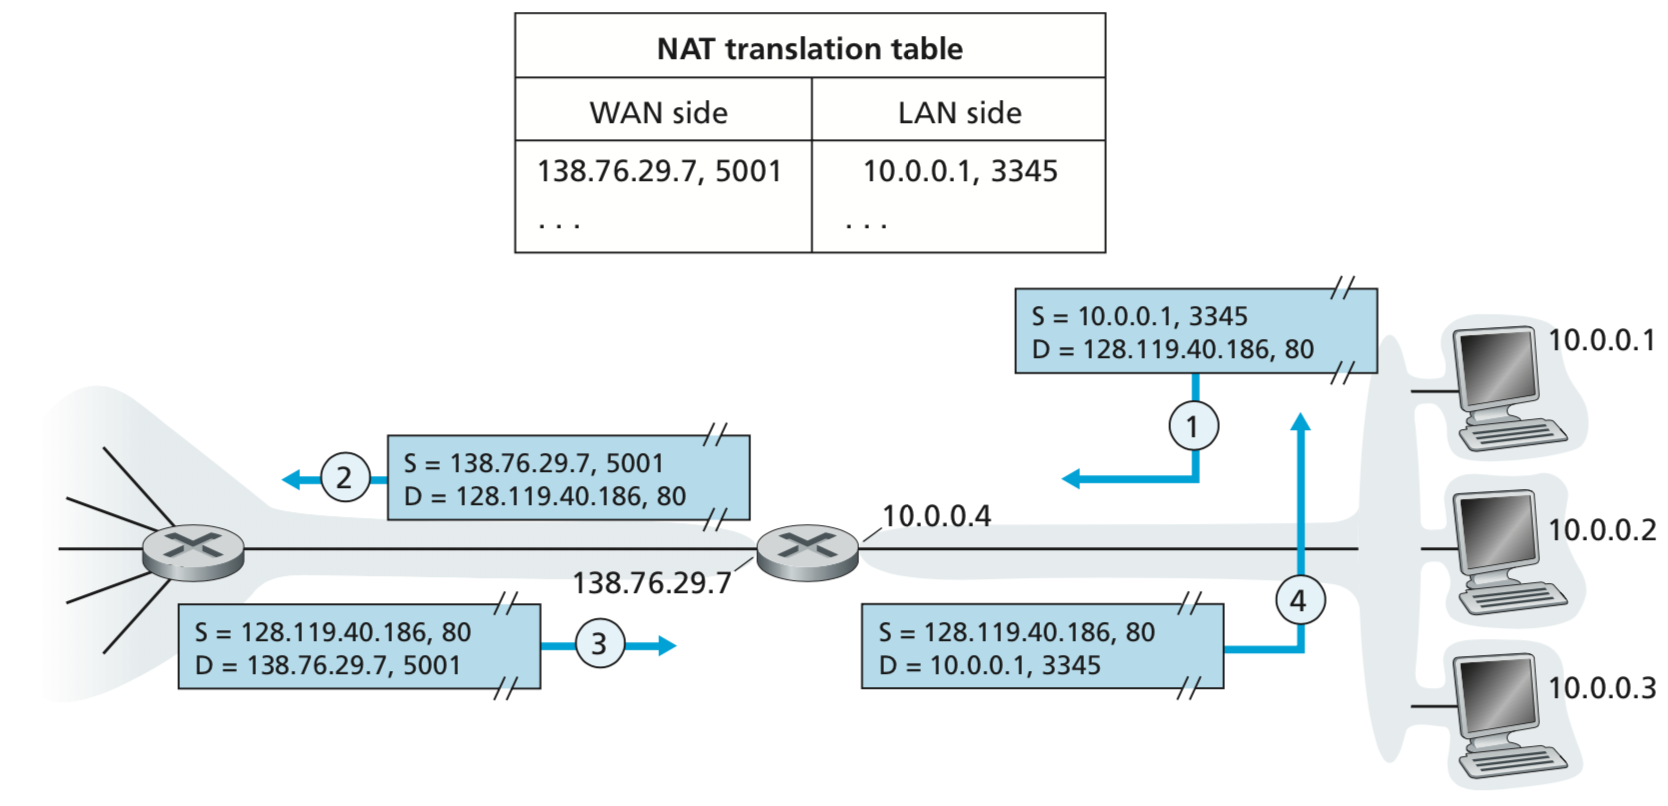
\includegraphics[width=0.8\linewidth]{images/NAT.png}
	\caption{Network address translation}
	\label{fig:NAT}
\end{figure}

\subsection{The Internet Protocol Version 6}

\begin{itemize}
	\item \textbf{Expanded addressing capabilities}
	
	IPv6 increases the size of the IP address from 32 to 128 bits. This ensures that the world won’t run out of IP addresses.
	
	\item \textbf{A streamlined 40-byte header}
	
	As discussed below, a number of IPv4 fields have been dropped or made optional. The resulting 40-byte fixed-length header allows for faster processing of the IP datagram by a router.
	
	\item \textbf{Flow labeling}
	
	IPv6 has an elusive definition of a flow.
	
\end{itemize}

\begin{figure}[h]
	\centering
	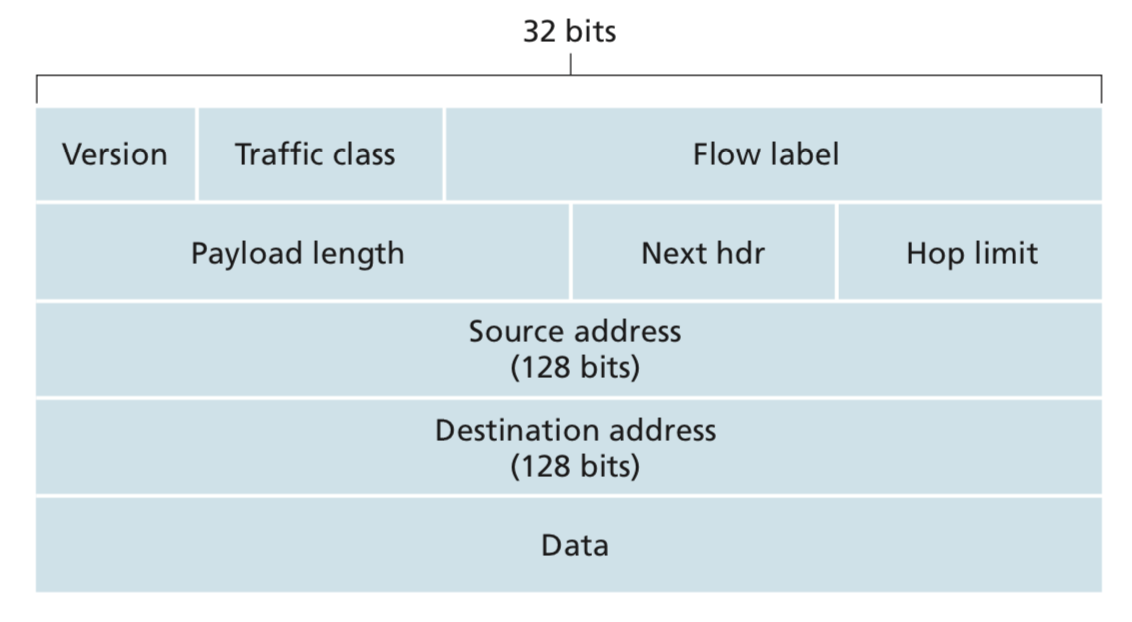
\includegraphics[width=0.8\linewidth]{images/ipv6.png}
	\caption{IPv6 datagram format}
	\label{fig:ipv6}
\end{figure}

\begin{itemize}
	\item \textbf{Version}
	
	This 4-bit field identifies the IP version number. Not surprisingly, IPv6 carries a value of 6 in this field. Note that putting a 4 in this field does not create a valid IPv4 datagram.
	
	\item \textbf{Traffic class}
	
	The 8-bit traffic class field, like the TOS field in IPv4, can be used to give priority to certain datagrams within a flow, or it can be used to give priority to datagrams from certain applications over datagrams from other applications
	
	\item \textbf{Flow label} 
	This 20-bit field is used to identify a flow of datagrams.
	
	\item \textbf{Payload length}
	
	This 16-bit value is treated as an unsigned integer giving the number of bytes in the IPv6 datagram following the fixed-length, 40-byte data- gram header.
	
	\item \textbf{Next header}
	
	This field identifies the protocol to which the contents (data field) of this datagram will be delivered (for example, to TCP or UDP). The field uses the same values as the protocol field in the IPv4 header.
	
	\item \textbf{Hop limit}
	
	The contents of this field are decremented by one by each router that forwards the datagram. If the hop limit count reaches zero, the datagram is discarded.
	
	\item \textbf{Source and destination addresses}
	
	\item \textbf{Data} 
	
	This is the payload portion of the IPv6 datagram. When the datagram reaches its destination, the payload will be removed from the IP datagram and passed on to the protocol specified in the next header field.
	
\end{itemize}

\subsection{Transitioning from IPv4 to IPv6}

\begin{figure}[h]
	\centering
	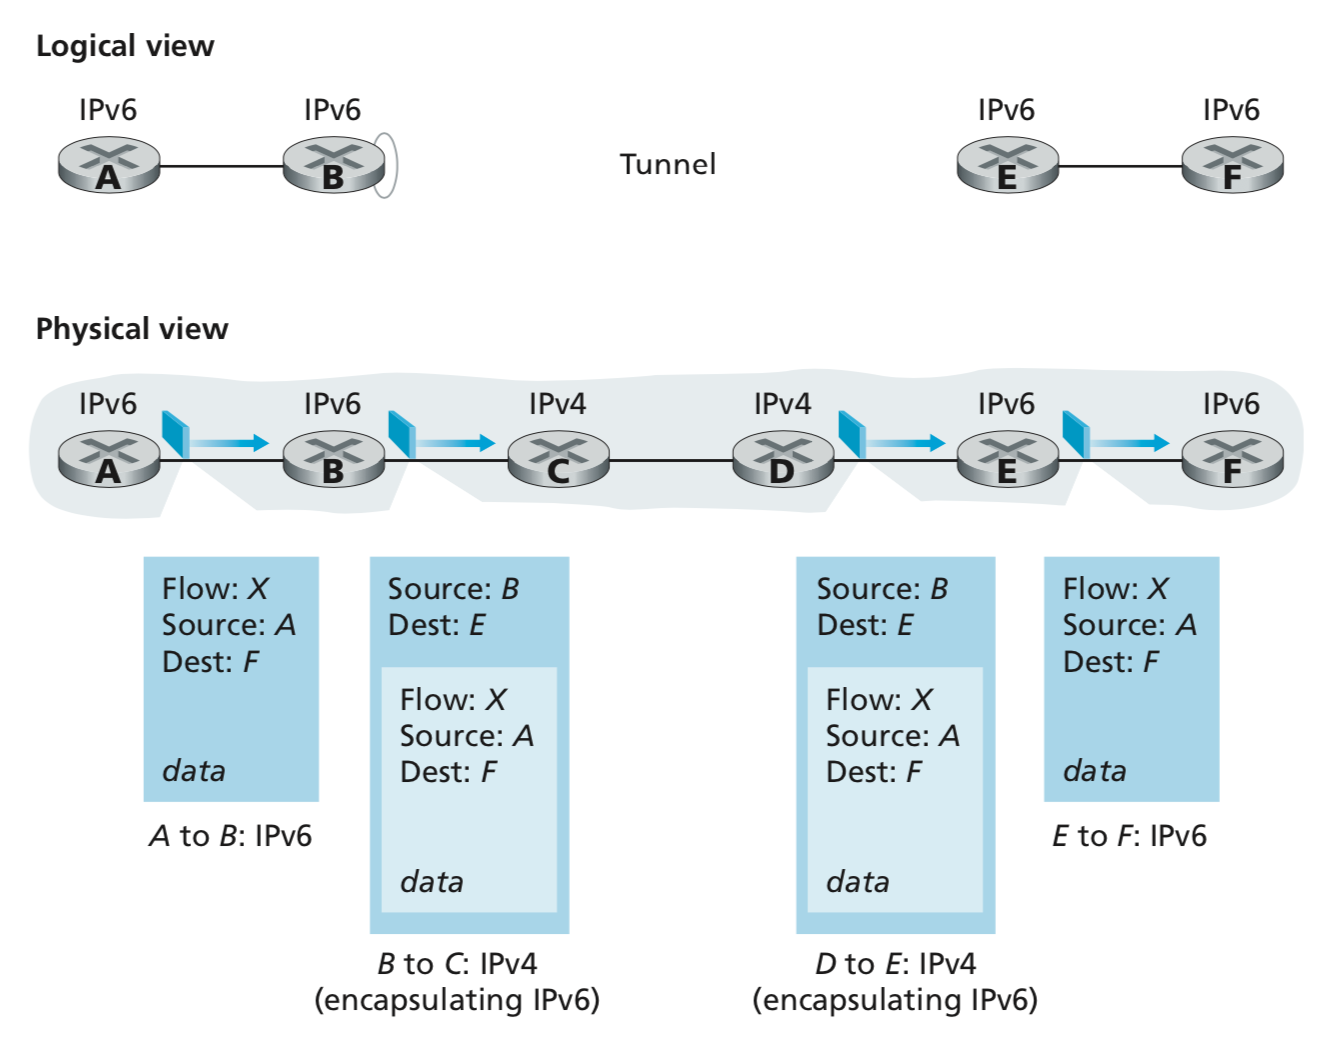
\includegraphics[width=0.8\linewidth]{images/Tunneling.png}
	\caption{Tunneling}
	\label{fig:Tunneling}
\end{figure}

\subsection{Routing Algorithms}

A \textbf{centralized routing algorithm} computes the least-cost path between a source and destination using complete, global knowledge about the network. Algorithms with global state information are often referred to as \textbf{link-state (LS) algorithms}, since the algorithm must be aware of the cost of each link in the network.

In a \textbf{decentralized routing algorithm}, the calculation of the least-cost path is carried out in an iterative, distributed manner by the routers. No node has complete information about the costs of all network links. Instead, each node begins with only the knowledge of the costs of its own directly attached links. Then, through an iterative process of calculation and exchange of information with its neighboring nodes, a node gradually calculates the least-cost path to a destination or set of destinations. \textbf{Distance-vector (DV) algorithm} is one of these algorithms.

A second broad way to classify routing algorithms is according to whether they are static or dynamic. In \textbf{static routing algorithms}, routes change very slowly over time, often as a result of human intervention (for example, a human manually editing a link costs). \textbf{Dynamic routing algorithms} change the routing paths as the network traffic loads or topology change. A dynamic algorithm can be run either periodically or in direct response to topology or link cost changes. While dynamic algorithms are more responsive to network changes, they are also more susceptible to problems such as routing loops and route oscillation.

A third way to classify routing algorithms is according to whether they are load-sensitive or load-insensitive. In a \textbf{load-sensitive algorithm}, link costs vary dynamically to reflect the current level of congestion in the underlying link. If a high cost is associated with a link that is currently congested, a routing algorithm will tend to choose routes around such a congested link. Today’s Internet routing algorithms are \textbf{load-insensitive}, as a link’s cost does not explicitly reflect its current (or recent past) level of congestion.

\begin{figure}[h]
	\centering
	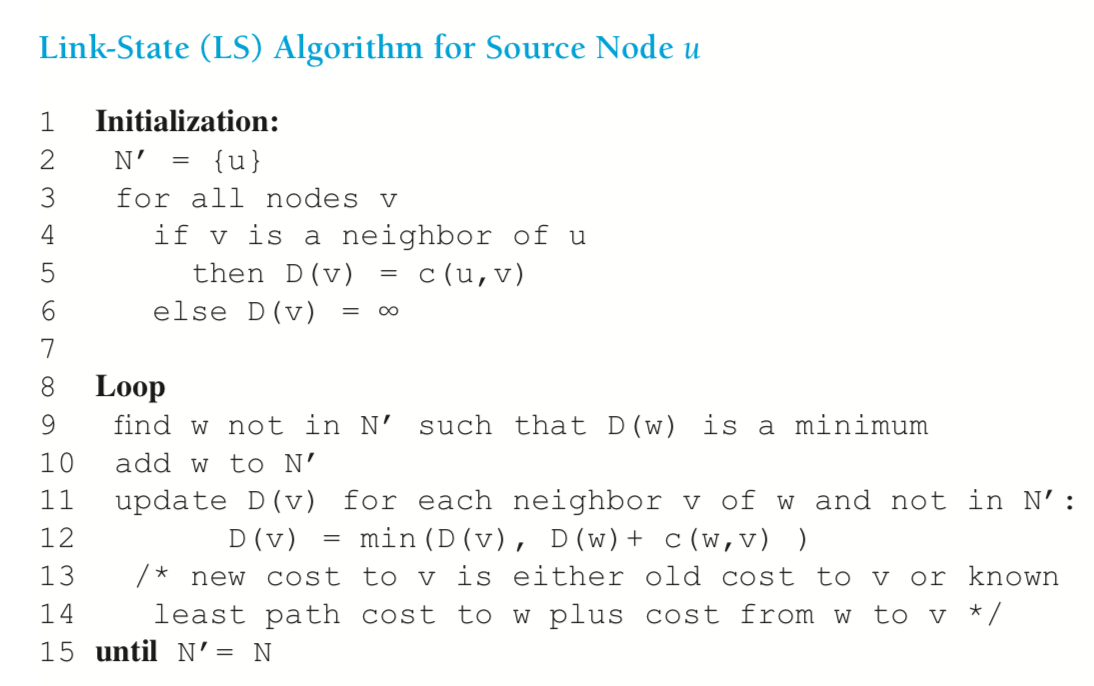
\includegraphics[width=0.8\linewidth]{images/ls.png}
	\caption{Link-State (LS) Algorithm for Source Node $u$}
	\label{fig:ls}
\end{figure}

\begin{figure}[h]
	\centering
	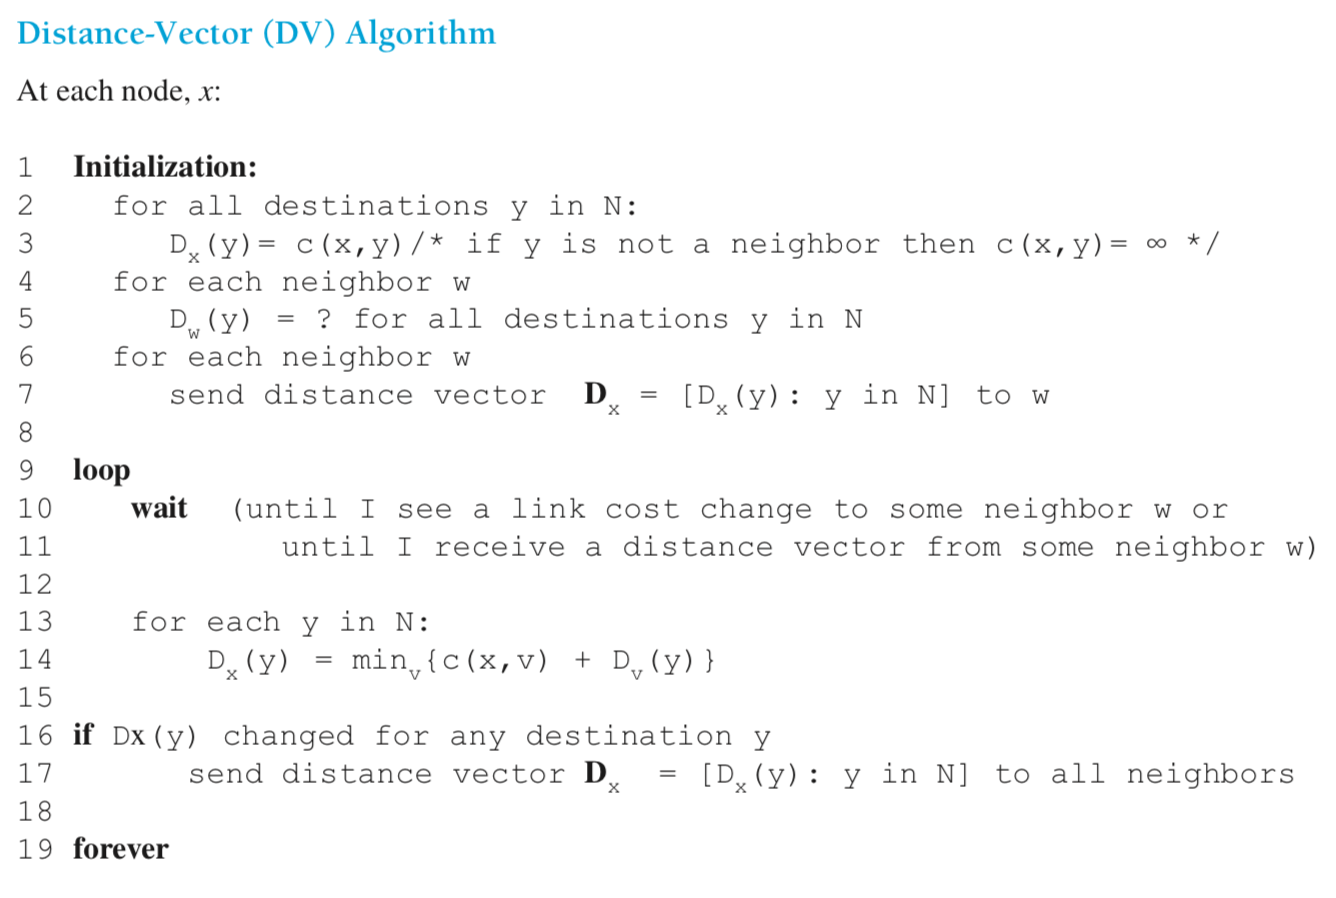
\includegraphics[width=0.8\linewidth]{images/dv.png}
	\caption{Distance-Vector (DV) Algorithm}
	\label{fig:dv}
\end{figure}

\subsection{Intra-AS Routing in the Internet : OSPF}

Each \textbf{autonomous systems (AS)} consisting of a group of routers that are under the same administrative control. An autonomous system is identified by its globally unique \textbf{autonomous system number (ASN)}. Routers within the same AS all run the same routing algorithm and have information about each other. The routing algorithm running within an autonomous system is called an \textbf{intra-autonomous system routing protocol}.

OSPF is a link-state protocol that uses flooding of link-state information and a Dijkstra’s least-cost path algorithm. With OSPF, each router constructs a complete topological map of the entire autonomous system. Each router then locally runs Dijkstra’s shortest-path algorithm to determine a shortest-path tree to all subnets, with itself as the root node. Individual link costs are configured by the network administrator.

\subsection{Routing Among the ISPs : BGP}

In fact, in the Internet, all ASs run the same \textbf{inter-autonomous system routing protocol}, called the \textbf{Border Gateway Protocol}, more commonly known as BGP. In BGP, packets are not routed to a specific destination address, but instead to CIDRized prefixes, with each prefix representing a subnet or a collection of subnets.

In \textbf{hot potato routing}, the route chosen (from among all possible routes) is that route with the least cost to the NEXT-HOP router beginning that route. 

\subsection{ICMP : The Internet Control Message Protocol}

The Internet Control Message Protocol (ICMP), is used by hosts and routers to communicate network-layer information to each other. 

\begin{figure}[h]
	\centering
	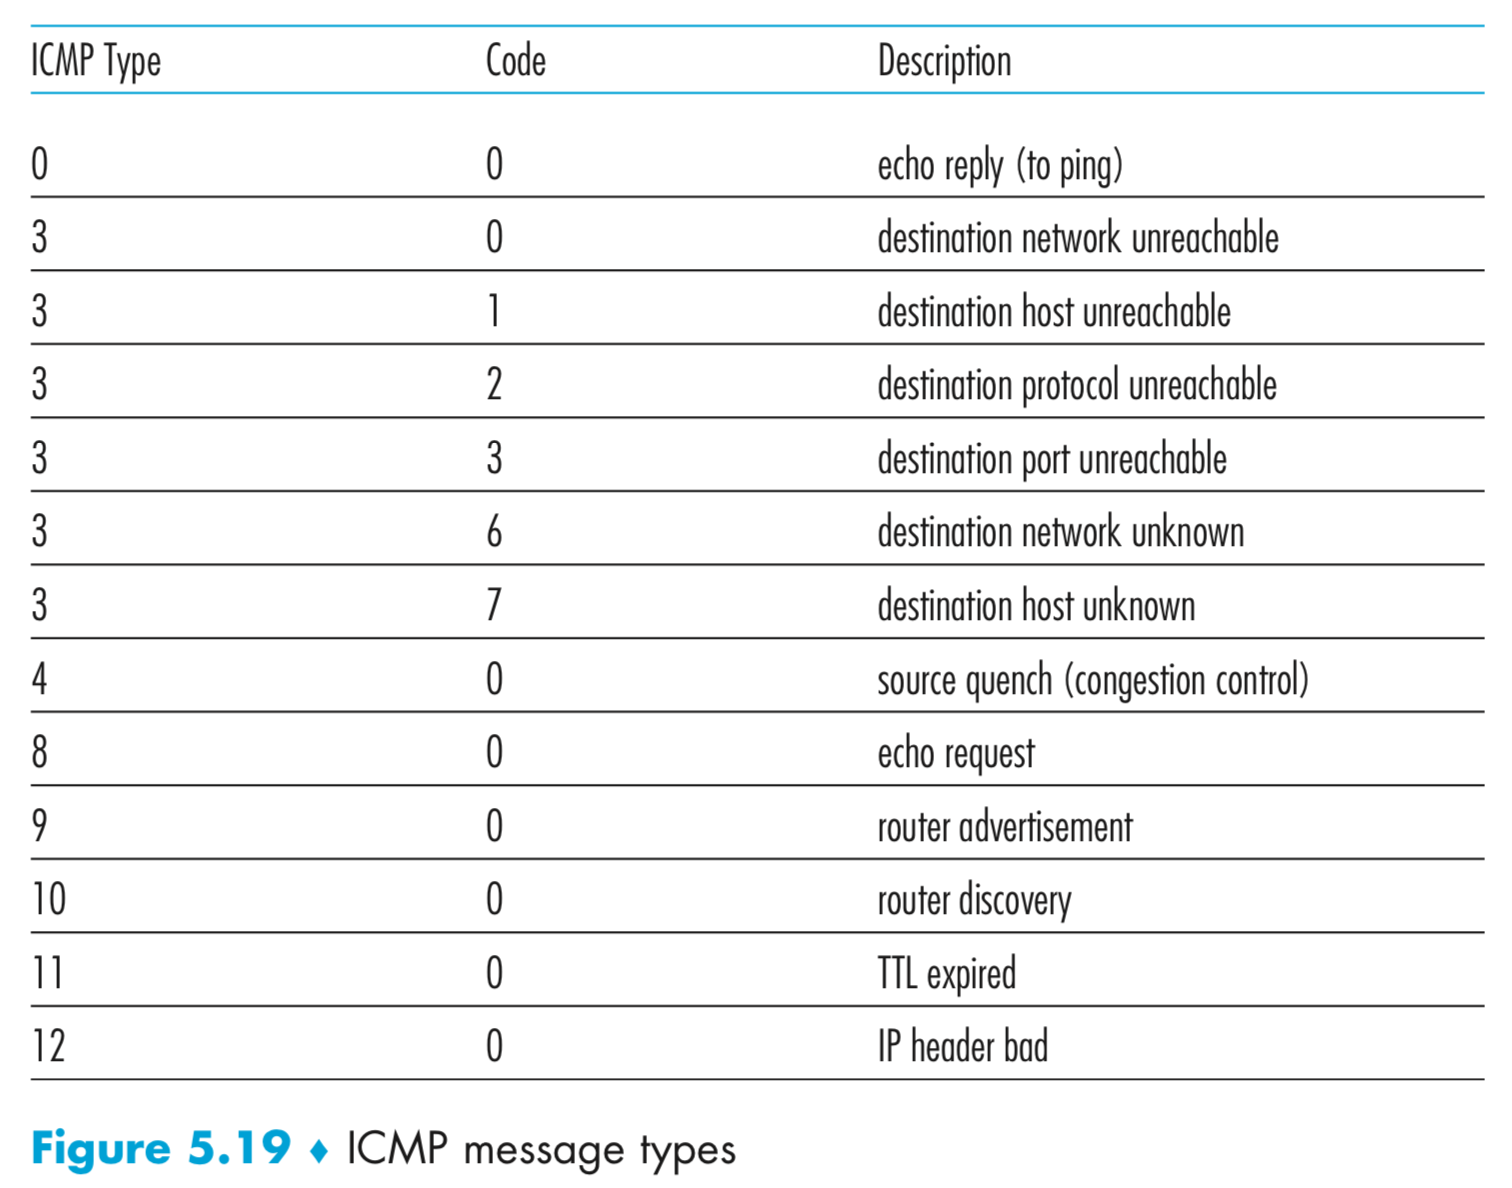
\includegraphics[width=0.8\linewidth]{images/ICMP.png}
	\caption{ICMP message types}
	\label{fig:ICMP}
\end{figure}

\section{Link Layer}

The Internet’s network layer routes a datagram through a series of routers between the source and destination. To move a packet from one node (host or router) to the next node in the route, the network layer relies on the services of the link layer.

\subsection{CRC : Cyclic Redundancy Check}

Consider the $d$-bit piece of data, $D$, that the sending node wants to send to the receiving node. The sender and receiver must first agree on an $r + 1$ bit pattern, known as a \textbf{generator}, which we will denote as $G$. We will require that the most significant (leftmost) bit of $G$ be a 1. The key idea behind CRC codes is shown in Figure \ref{fig:CRC}. For a given piece of data, $D$, the sender will choose $r$ additional bits, $R$, and append them to $D$ such that the resulting $d + r$ bit pattern (interpreted as a binary number) is exactly divisible by $G$ (i.e., has no remainder) using modulo-2 arithmetic. The process of error checking with CRCs is thus simple: The receiver divides the $d + r$ received bits by $G$. If the remainder is nonzero, the receiver knows that an error has occurred; otherwise the data is accepted as being correct. All CRC calculations are done in modulo-2 arithmetic without carries in addition or borrows in subtraction. This means that addition and subtraction are identical, and both are equivalent to the bitwise exclusive-or (XOR) of the operands. 

\begin{figure}[h]
	\centering
	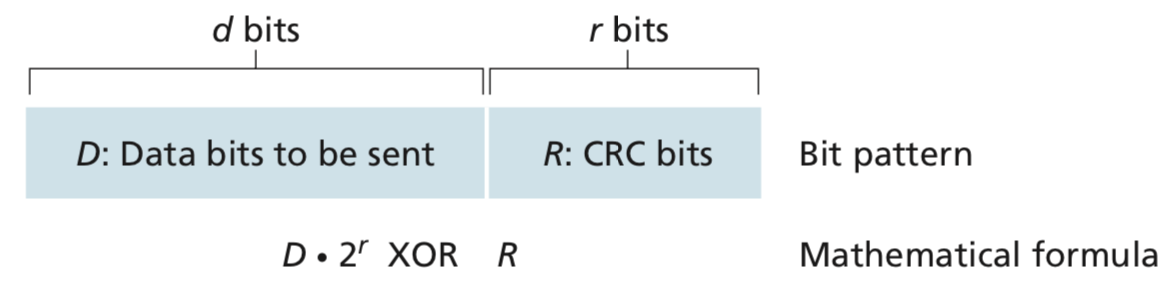
\includegraphics[width=0.7\linewidth]{images/CRC.png}
	\caption{CRC}
	\label{fig:CRC}
\end{figure}

$R$ can be computed as follows, 
\[
	R = \mathrm{remainder} \frac{D \cdot 2^r}{G}
\]

\begin{figure}[h]
	\centering
	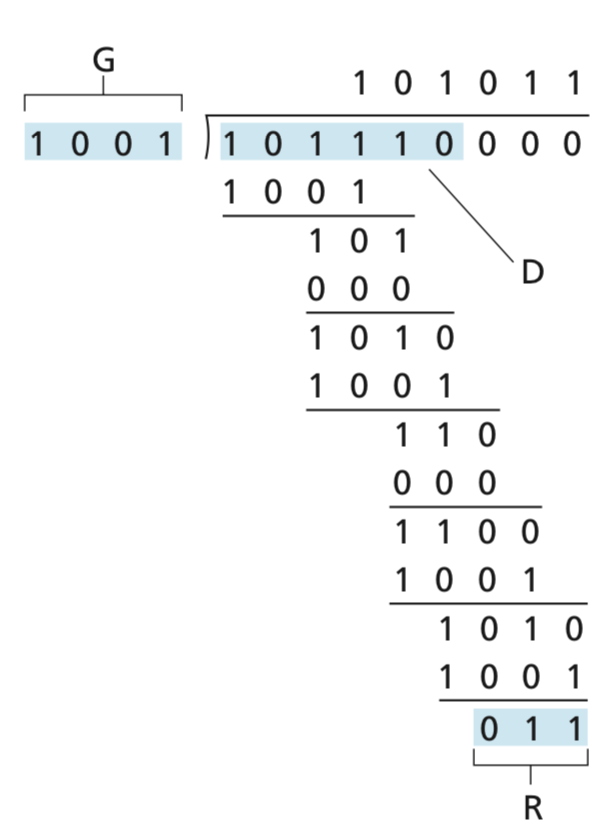
\includegraphics[width=0.5\linewidth]{images/CRCC.png}
	\caption{A sample CRC calculation}
	\label{fig:CRCC}
\end{figure}

\subsection{Random Access Protocols}

In a random access protocol, a transmitting node always transmits at the full rate of the channel, namely, $R$ bps. When there is a collision, each node involved in the collision repeatedly retransmits its frame until its frame gets through without a collision. But when a node experiences a collision, it doesn’t necessarily retransmit the frame right away. Instead it waits a random delay before retransmitting the frame. Each node involved in a collision chooses independent random delays. 

\subsubsection{Slotted ALOHA}

In our description of slotted ALOHA, we assume the following:

\begin{itemize}
	\item All frames consist of exactly $L$ bits.
	
	\item Time is divided into slots of size $\frac{L}{R}$ seconds (that is, a slot equals the time to transmit one frame).
	
	\item Nodes start to transmit frames only at the beginnings of slots.
	
	\item The nodes are synchronized so that each node knows when the slots begin.
	
	\item If two or more frames collide in a slot, then all the nodes detect the collision event before the slot ends.
\end{itemize}

Let $p$ be a probability, that is, a number between 0 and 1. The operation of slotted ALOHA in each node is simple:

\begin{itemize}
	\item When the node has a fresh frame to send, it waits until the beginning of the next slot and transmits the entire frame in the slot.
	
	\item If there isn’t a collision, the node has successfully transmitted its frame and thus need not consider retransmitting the frame. (The node can prepare a new frame for transmission, if it has one.)
	
	\item If there is a collision, the node detects the collision before the end of the slot. The node retransmits its frame in each subsequent slot with probability $p$ until the frame is transmitted without a collision.

\end{itemize}

Suppose there are $N$ nodes. Then the probability that a given slot is a successful slot is the probability that one of the nodes transmits and that the remaining $N - 1$ nodes do not transmit. The probability that a given node transmits is $p$; the probability that the remaining nodes do not transmit is $(1 - p)^{N-1}$. Therefore the probability a given node has a success is $p(1 - p)^{N-1}$. Because there are $N$ nodes, the probability that any one of the $N$ nodes has a success is $Np(1 - p)^{N - 1}$.

\subsection{CSMA : Carrier Sense Multiple Access}

\subsubsection{Characteristic}

\begin{itemize}
	\item  \textbf{Carrier Sensing}
	
	A node listens to the channel before transmitting. If a frame from another node is currently being transmitted into the channel, a node then waits until it detects no transmissions for a short amount of time and then begins transmission.
	
	\item \textbf{Collision detection}
	
	A transmitting node listens to the channel while it is transmitting. If it detects that another node is transmitting an interfering frame, it stops transmitting and waits a random amount of time before repeating the sense-and-transmit-when-idle cycle.
	
\end{itemize}

\subsubsection{Operations from the Perspective of an Node}

\begin{enumerate}

	\item The adapter obtains a datagram from the network layer, prepares a link-layer frame, and puts the frame adapter buffer.
	\item If the adapter senses that the channel is idle (that is, there is no signal energy entering the adapter from the channel), it starts to transmit the frame. If, on the other hand, the adapter senses that the channel is busy, it waits until it senses no signal energy and then starts to transmit the frame.
	
	\item While transmitting, the adapter monitors for the presence of signal energy coming from other adapters using the broadcast channel.
	
	\item If the adapter transmits the entire frame without detecting signal energy from other adapters, the adapter is finished with the frame. If, on the other hand, the adapter detects signal energy from other adapters while transmitting, it aborts the transmission (that is, it stops transmitting its frame).
	
	\item After aborting, the adapter waits a random amount of time and then returns to step 2.
\end{enumerate}

\subsubsection{Binary Exponential Backoff Algorithm}
When transmitting a frame that has already experienced $n$ collisions, a node chooses the value of $K$ at random from $\{0,1,2, . . . . 2^{n-1}\}$. Thus, the more collisions experienced by a frame, the larger the interval from which $K$ is chosen.

\subsubsection{Efficiency}

Let $d_{prop}$ denote the maximum time it takes signal energy to propagate between any two adapters. Let $d_{trans}$ be the time to transmit a maximum-size frame. Here we simply state the following approximation:

\[
	\mathrm{Efficiency} = \frac{1}{1 + 5 \frac{d_{prop}}{d_{trans}}}
\]

We see from this formula that as $d_{prop}$ approaches 0, the efficiency approaches 1. This matches our intuition that if the propagation delay is zero, colliding nodes will abort immediately without wasting the channel. Also, as $d_{trans}$ becomes very large, efficiency approaches 1. This is also intuitive because when a frame grabs the channel, it will hold on to the channel for a very long time; thus, the channel will be doing productive work most of the time.

\subsection{Taking-Turns Protocols}

\subsubsection{Polling Protocol}

The first one is the polling protocol. The polling protocol requires one of the nodes to be designated as a master node. The master node polls each of the nodes in a round-robin fashion. In particular, the master node first sends a message to node 1, saying that it (node 1) can transmit up to some maximum number of frames. After node 1 transmits some frames, the master node tells node 2 it (node 2) can transmit up to the maximum number of frames. The procedure continues in this manner, with the master node polling each of the nodes in a cyclic manner.

\subsubsection{Token-Passing Protocol}

In this protocol there is no master node. A small, special-purpose frame known as a token is exchanged among the nodes in some fixed order. For example, node 1 might always send the token to node 2, node 2 might always send the token to node 3, and node $N$ might always send the token to node 1. When a node receives a token, it holds onto the token only if it has some frames to transmit; otherwise, it immediately forwards the token to the next node. If a node does have frames to transmit when it receives the token, it sends up to a maximum number of frames and then forwards the token to the next node. 

\subsection{MAC Addresses}

A link-layer address is variously called a \textbf{LAN address}, a \textbf{physical address}, or a \textbf{MAC address}. Because MAC address seems to be the most popular term, we’ll henceforth refer to link-layer addresses as MAC addresses. The MAC address is 6 bytes long, giving 248 possible MAC addresses. The \textbf{broadcast address} is a string of 48 consecutive 1s (that is, FF-FF-FF-FF-FF-FF in hexadecimal notation).

\subsection{ARP : Address Resolution Protocol}

ARP resolves IP addresses only for hosts and router interfaces on the same subnet. Each host and router has an ARP table in its memory, which contains mappings of IP addresses to MAC addresses. An \textbf{ARP packet} has several fields, including the sending and receiving IP and MAC addresses. Both ARP query and response packets have the same format. The purpose of the ARP query packet is to query all the other hosts and routers on the subnet to determine the MAC address corresponding to the IP address that is being resolved.

\section{Terminology}

\begin{itemize}

	\item \textbf{RTT : Round-Trip Time}
	
	\item \textbf{MSS : Maximum Segment Size}
	
	\item \textbf{MTU : Maximum Transmission Unit}
	
	\item \textbf{SDN : Software-Defined Networking}

\end{itemize}

\end{document}